\documentclass[10pt]{beamer}
\usetheme{Rochester}
\usepackage[utf8]{inputenc}
\usepackage{amsmath}
\usepackage{amsfonts}
\usepackage{amssymb}
\usepackage[export]{adjustbox}
\usepackage{efbox}
\usepackage{xcolor,colortbl}
\usepackage{transparent}
\usepackage[compat=1.0.0]{tikz-feynman}
\setbeamertemplate{footline}[frame number]
\definecolor{emerald}{rgb}{0.31, 0.78, 0.47}
\definecolor{lightblue}{rgb}{0.63, 0.79, 0.95}
\usepackage{siunitx}
\author{Justin Anguiano}

\title{Study of $WW\rightarrow qql\nu$ at the ILC}
%\setbeamercovered{transparent} 
%\setbeamertemplate{navigation symbols}{} 
%\logo{} 
\institute{University Of Kansas} 
\date{\today} 
%\subject{} 
\setbeamertemplate{navigation symbols}{}
\begin{document}
\maketitle


\begin{frame}
\tableofcontents
\end{frame}
\begin{frame}{What is the ILC?}
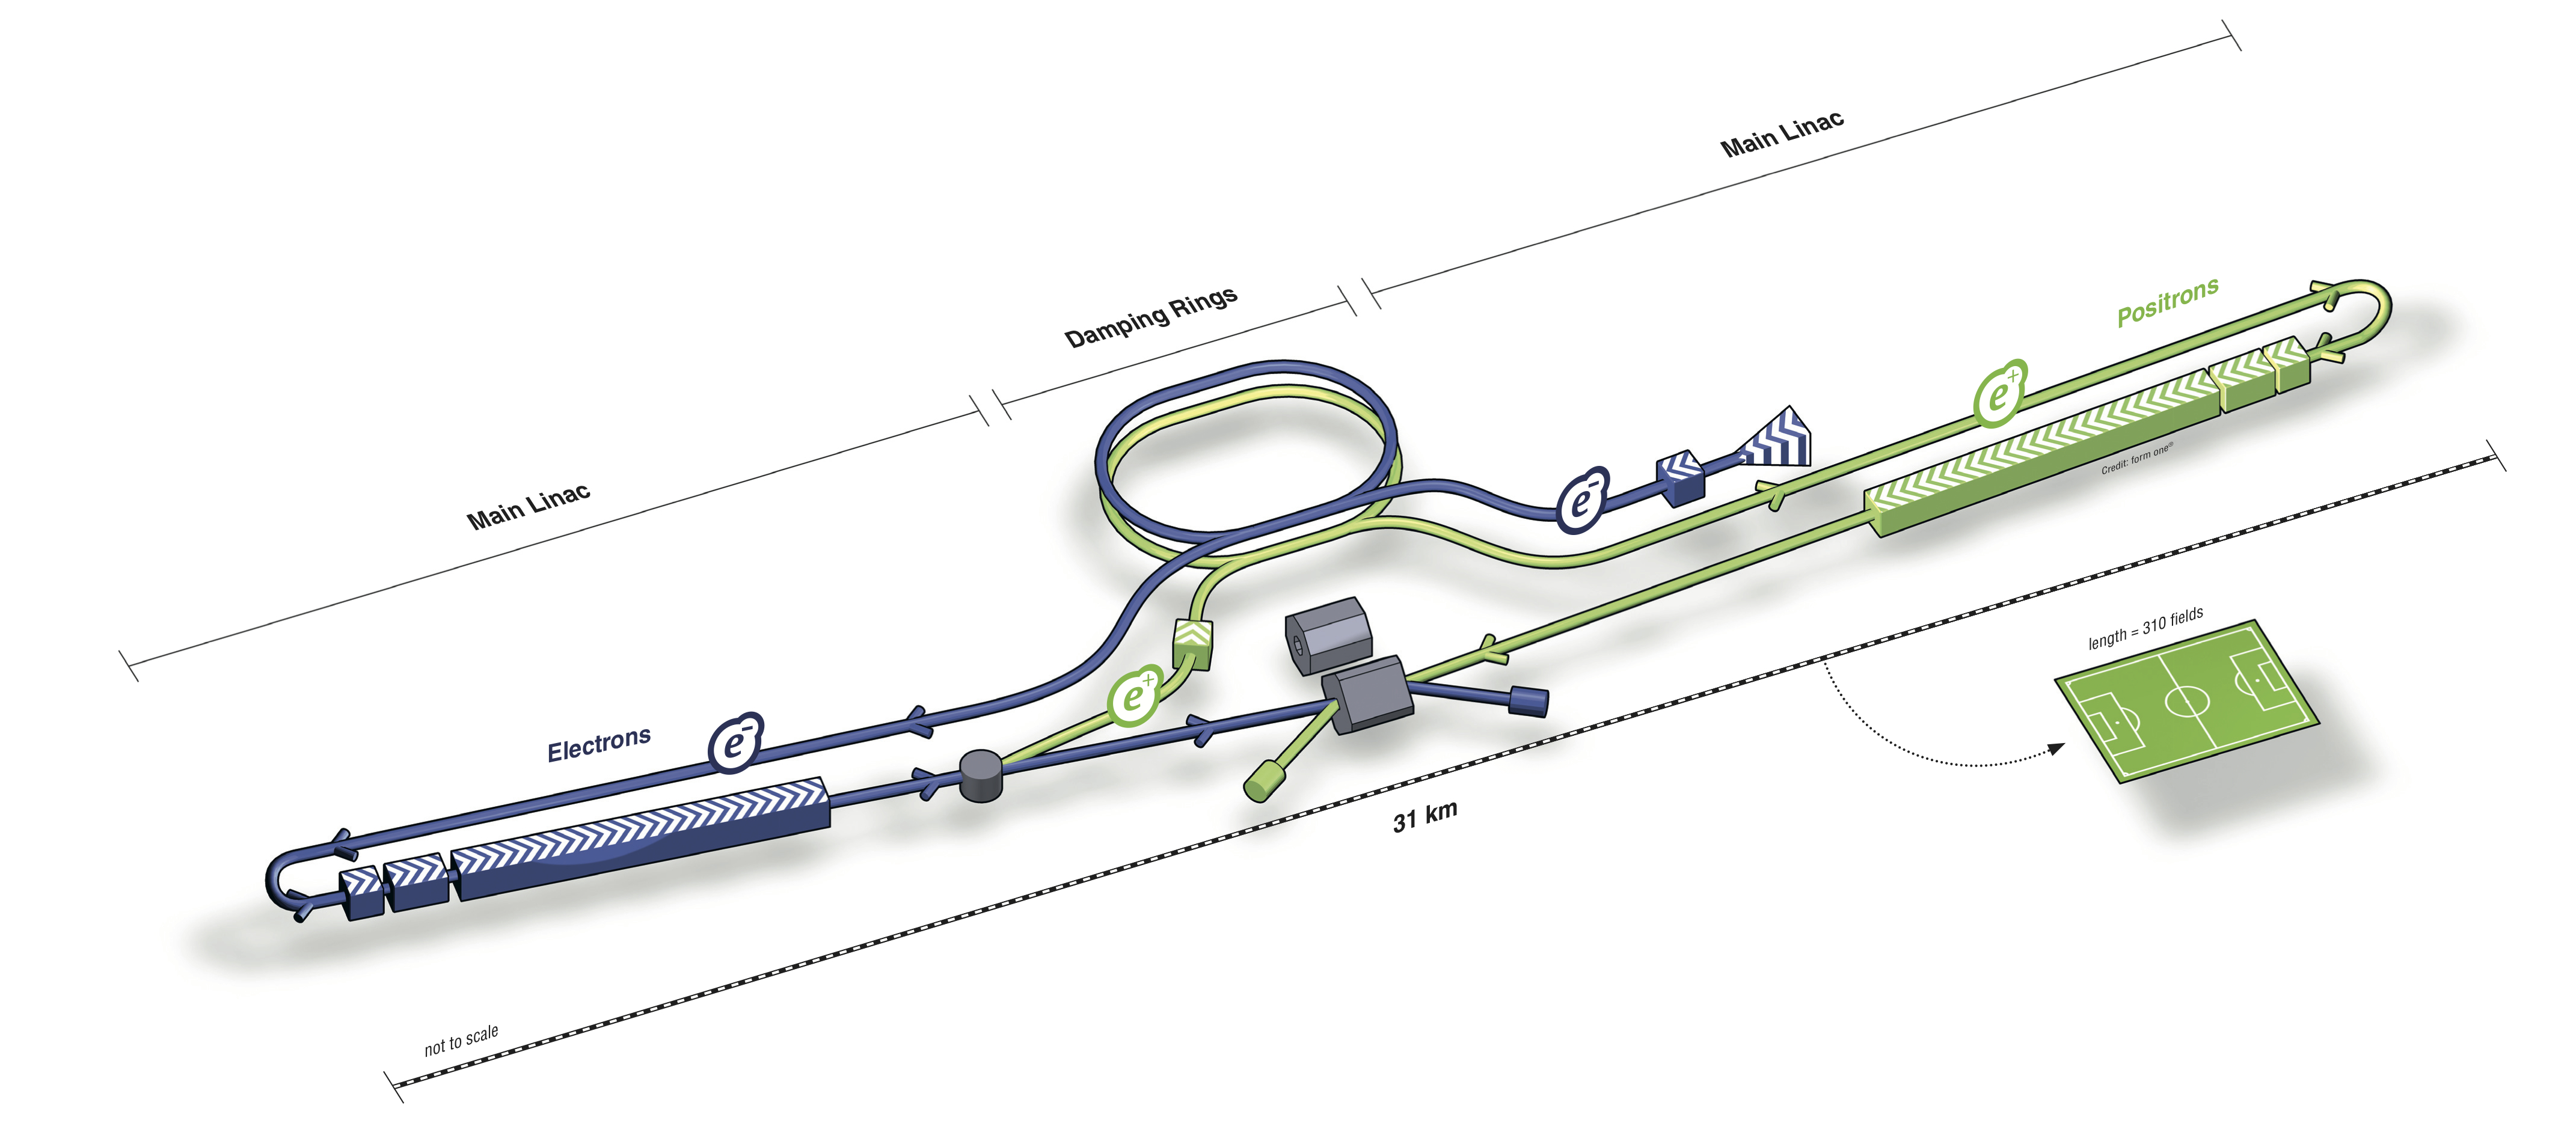
\includegraphics[scale=0.25]{ilcconcept.jpg}\\
\begin{columns}
\begin{column}{0.5\textwidth}
\begin{itemize}
\scriptsize
\item A new  $e^+ e^-$ linear collider 
\item Proposed cite in Japan 
\item Center of mass energy  250 GeV? 500 GeV? 0 GeV? -- up to 1 TeV?
\item Has tunable longitudinally polarized beams
\item Single IP serviced by 2 detectors
\item Currently in political limbo, will it get built???
\end{itemize}
\end{column}
\begin{column}{0.5\textwidth}
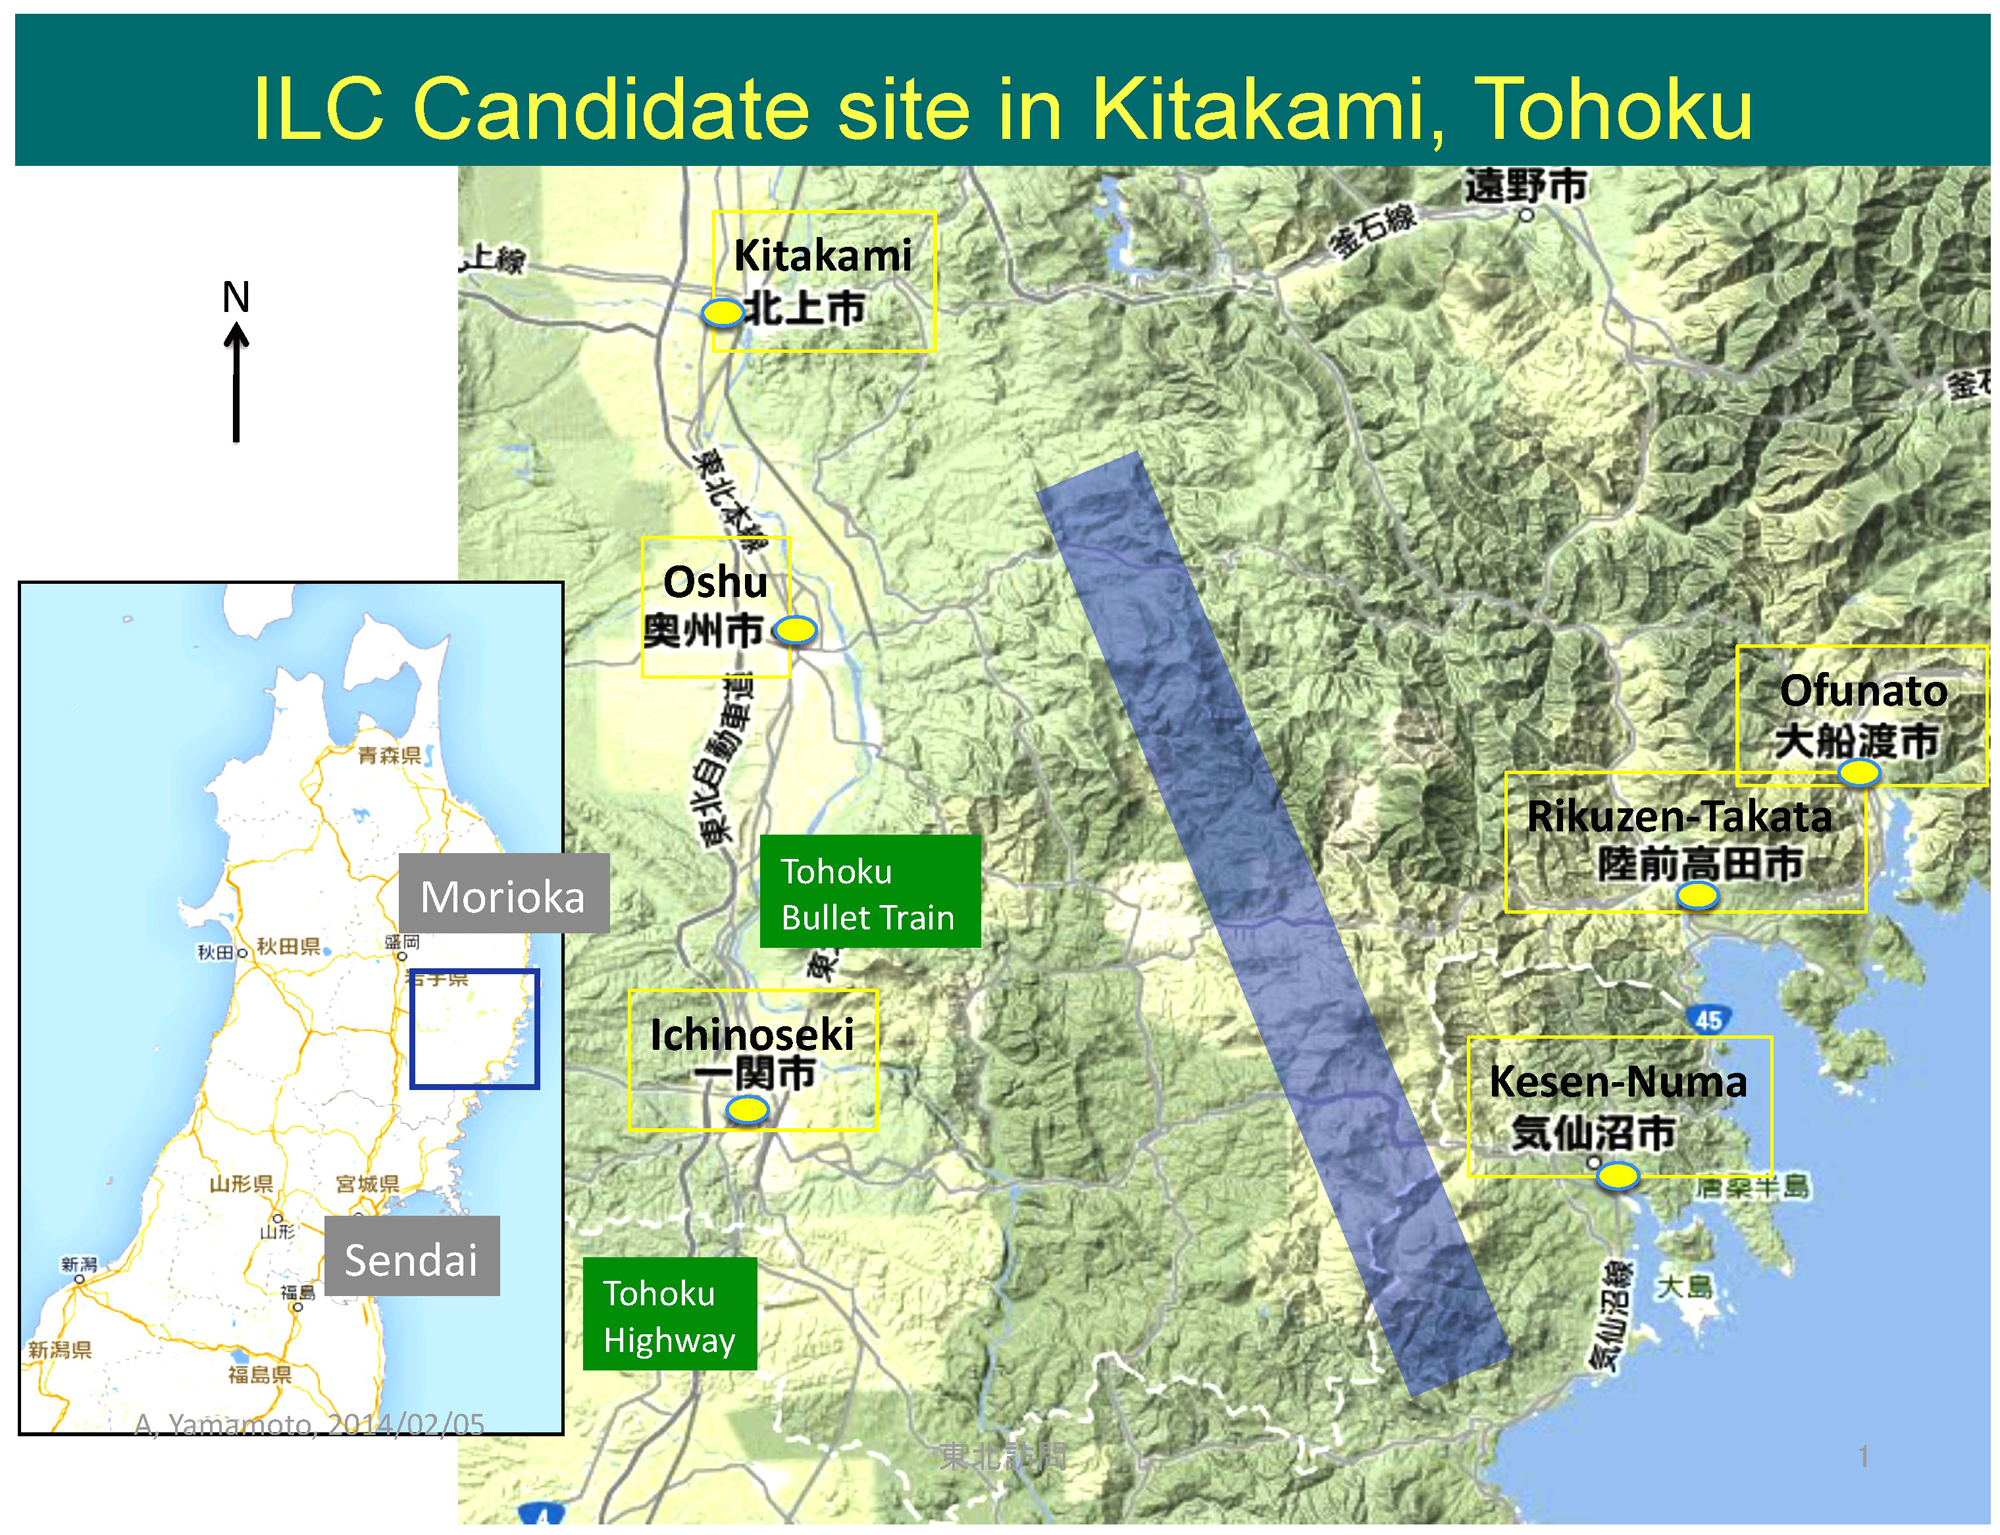
\includegraphics[scale=0.3]{ILC-Candidate-Area2.jpg}\\

\end{column}
\end{columns}s
\end{frame}

\begin{frame}{History of ILC}
Google Trends ``International Linear Collider" 2004-Present
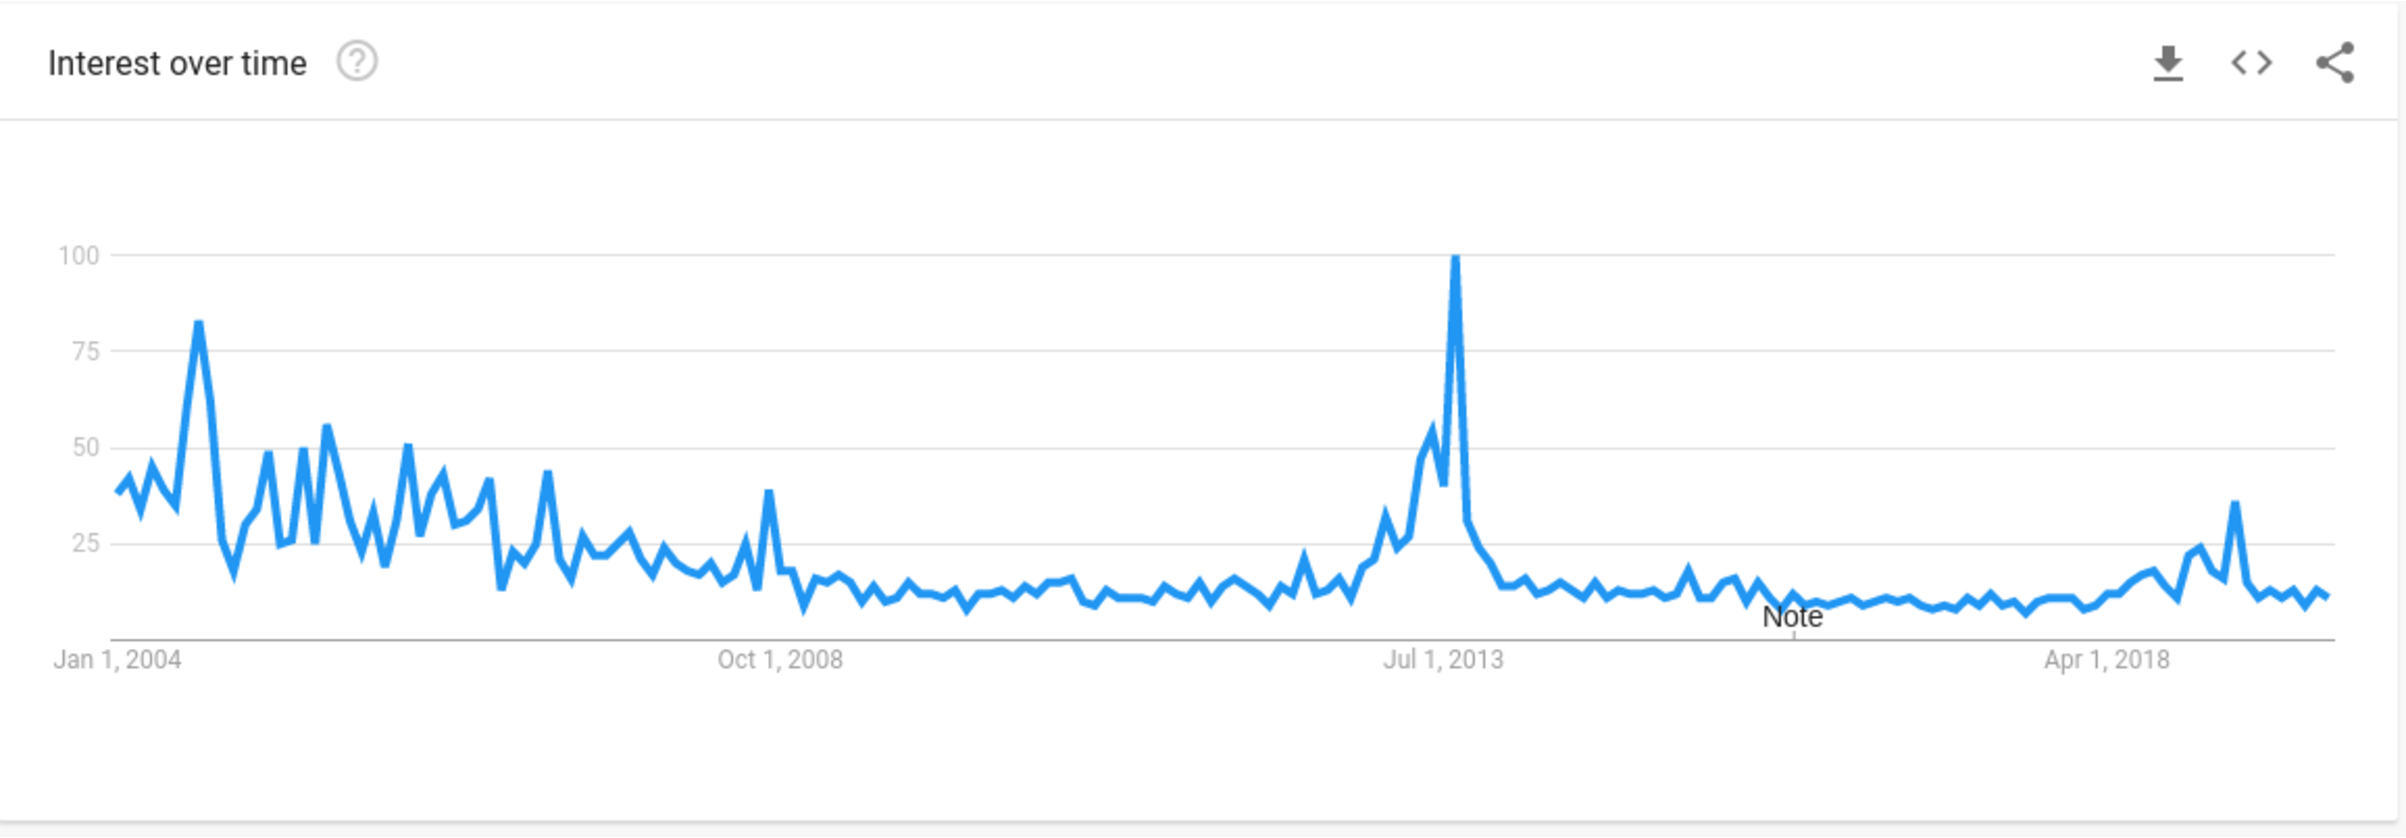
\includegraphics[scale=0.25]{ilctrends.pdf}\\
\begin{columns}
\begin{column}{0.5\textwidth}
\begin{itemize}
\scriptsize
\item Origins predate Google history starting in 2004
\item Linear collider discussed as next step for HEP as early as 1978
\item Many early competing proposals: TESLA, NLC, CLIC, GLC, SLC (1994)
\item ILC born from consolidating many proposals $\sim 2001$
\end{itemize}
\end{column}
\begin{column}{0.5\textwidth}
\includegraphics[scale=0.03]{futureaccel.png}\\
\end{column}
\end{columns}
\end{frame}

\begin{frame}{History of ILC}
Google Trends ``International Linear Collider" 2004-Present
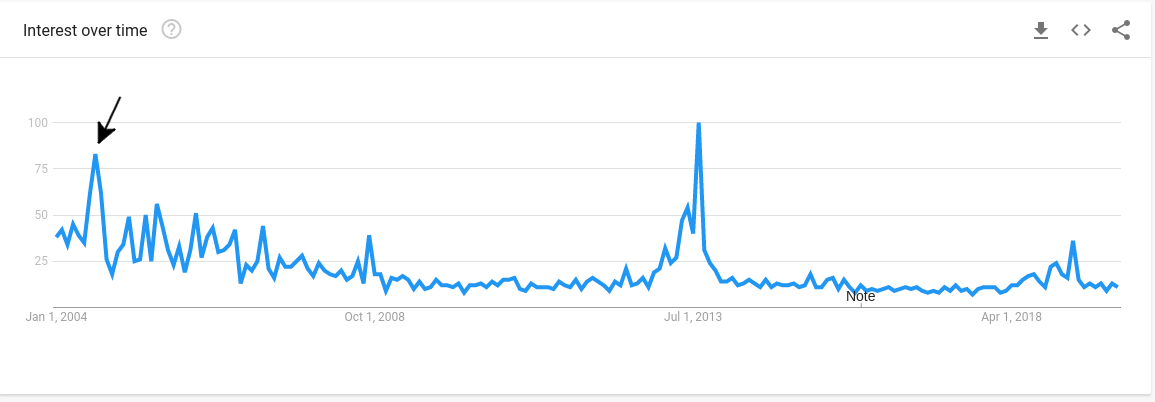
\includegraphics[scale=0.25]{timeline1.png}\\
August 2004 
\begin{itemize}
\scriptsize
\item the International Technology Recommendation Panel (ITRP) recommended a superconducting radio frequency technology for the accelerator. 

\item This decision causes – the Next Linear Collider (NLC), the Global Linear Collider (GLC) and Teraelectronvolt Energy Superconducting Linear Accelerator (TESLA) -- to join their efforts (ILC)
\end{itemize}
\end{frame}
\begin{frame}{History of ILC}
Google Trends ``International Linear Collider" 2004-Present
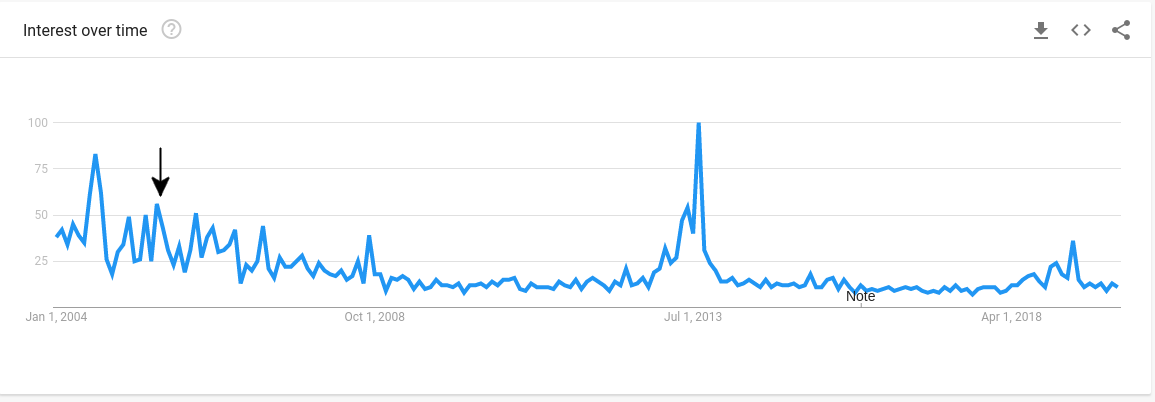
\includegraphics[scale=0.25]{timeline2.png}\\
\begin{columns}
\begin{column}{0.5\textwidth}

August 2005 
\begin{itemize}
\scriptsize
\item 2nd ILC Workshop, Snowmass Colorado -- earliest web-documented planning for the development of the ILC 

\item LCnewsline founded, dedicated resource for news, milestones, and developments related to ILC
\item No official host cite yet..
\end{itemize}
\end{column}
\begin{column}{0.5\textwidth}

\includegraphics[scale=0.2]{lcnews.png}\\

\end{column}
\end{columns}
\end{frame}
\begin{frame}{History of ILC}
Google Trends ``International Linear Collider" 2004-Present
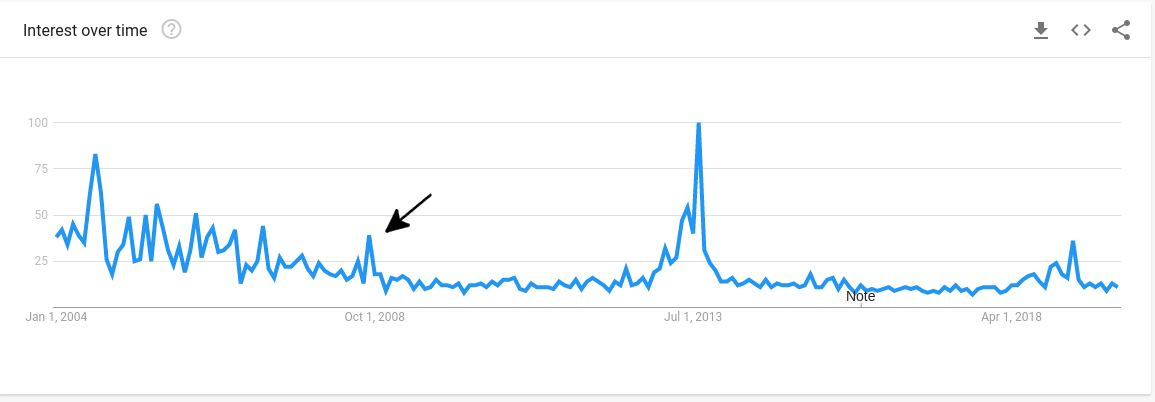
\includegraphics[scale=0.25]{timeline3.png}\\
September 2008 
\begin{itemize}
\item High Energy Physics in Philadelphia — ICHEP 08 
\item Open house at KEK, Japan expresses interest in hosting ILC
\end{itemize} 
\end{frame}
\begin{frame}{History of ILC}
Google Trends ``International Linear Collider" 2004-Present
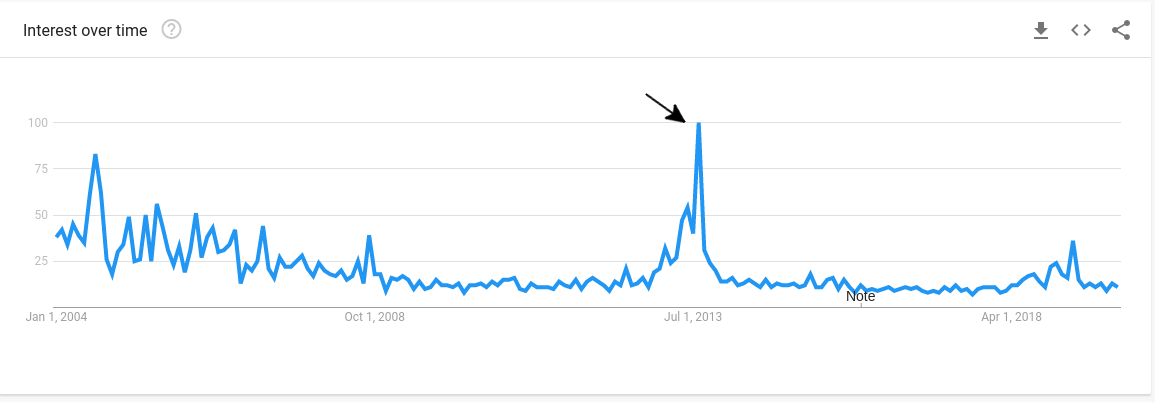
\includegraphics[scale=0.25]{timeline4.png}\\
August 2013 
\begin{columns}
\begin{column}{0.5\textwidth}
\begin{itemize}
\scriptsize
\item Japan announces candidate site for the ILC (Tohoku)
\item Still expresses ``interest in hosting" not guaranteeing hosting
\end{itemize}
\end{column}
\begin{column}{0.5\textwidth}
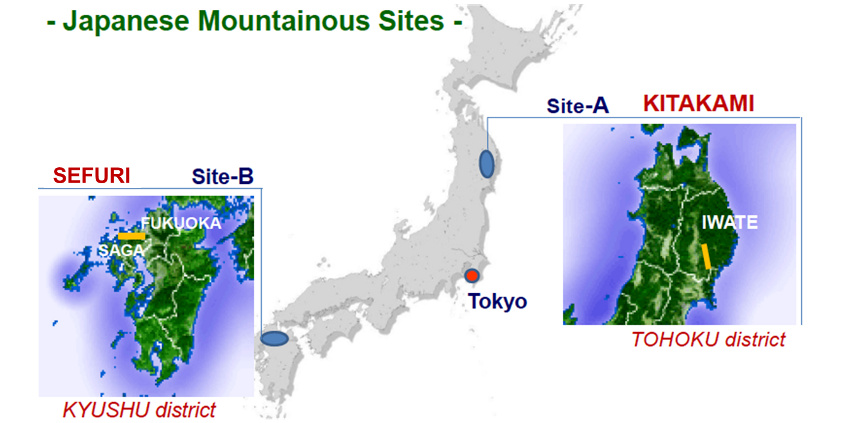
\includegraphics[scale=0.2]{japanese_sites.jpg}\\
\end{column}
\end{columns}

\end{frame}
\begin{frame}{History of ILC}
Google Trends ``International Linear Collider" 2004-Present
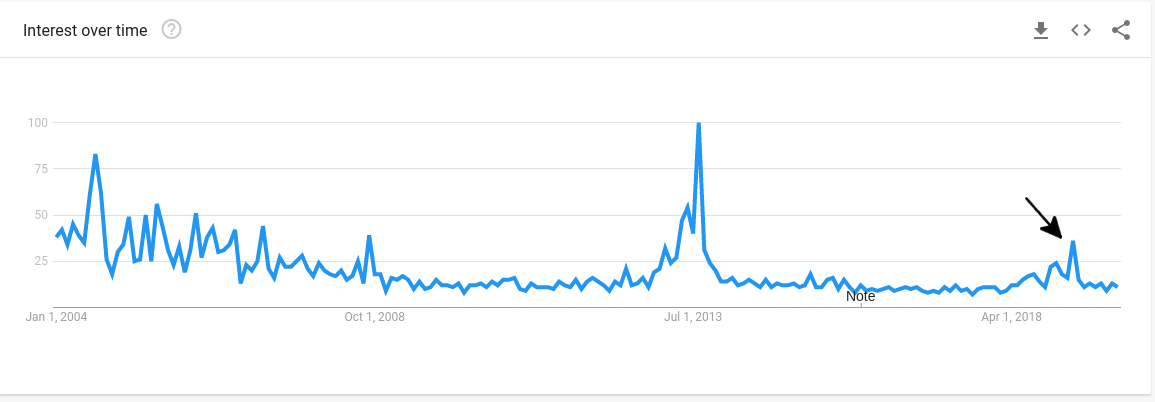
\includegraphics[scale=0.25]{timeline5.png}\\
March 2019
\begin{itemize}
\item ``The government has decided to not yet make a proposal to host the project, but has expressed interest in the ILC project and signalled to continue discussing it with other governments."
\item Progress continues crawling forward
\item Officially hosting requires negotiating costs with other governments
\end{itemize}
\end{frame}

\begin{frame}{ILC Detector the ILD }
The International Large Detector (ILD)\\
\begin{columns}
\begin{column}{0.5\textwidth}
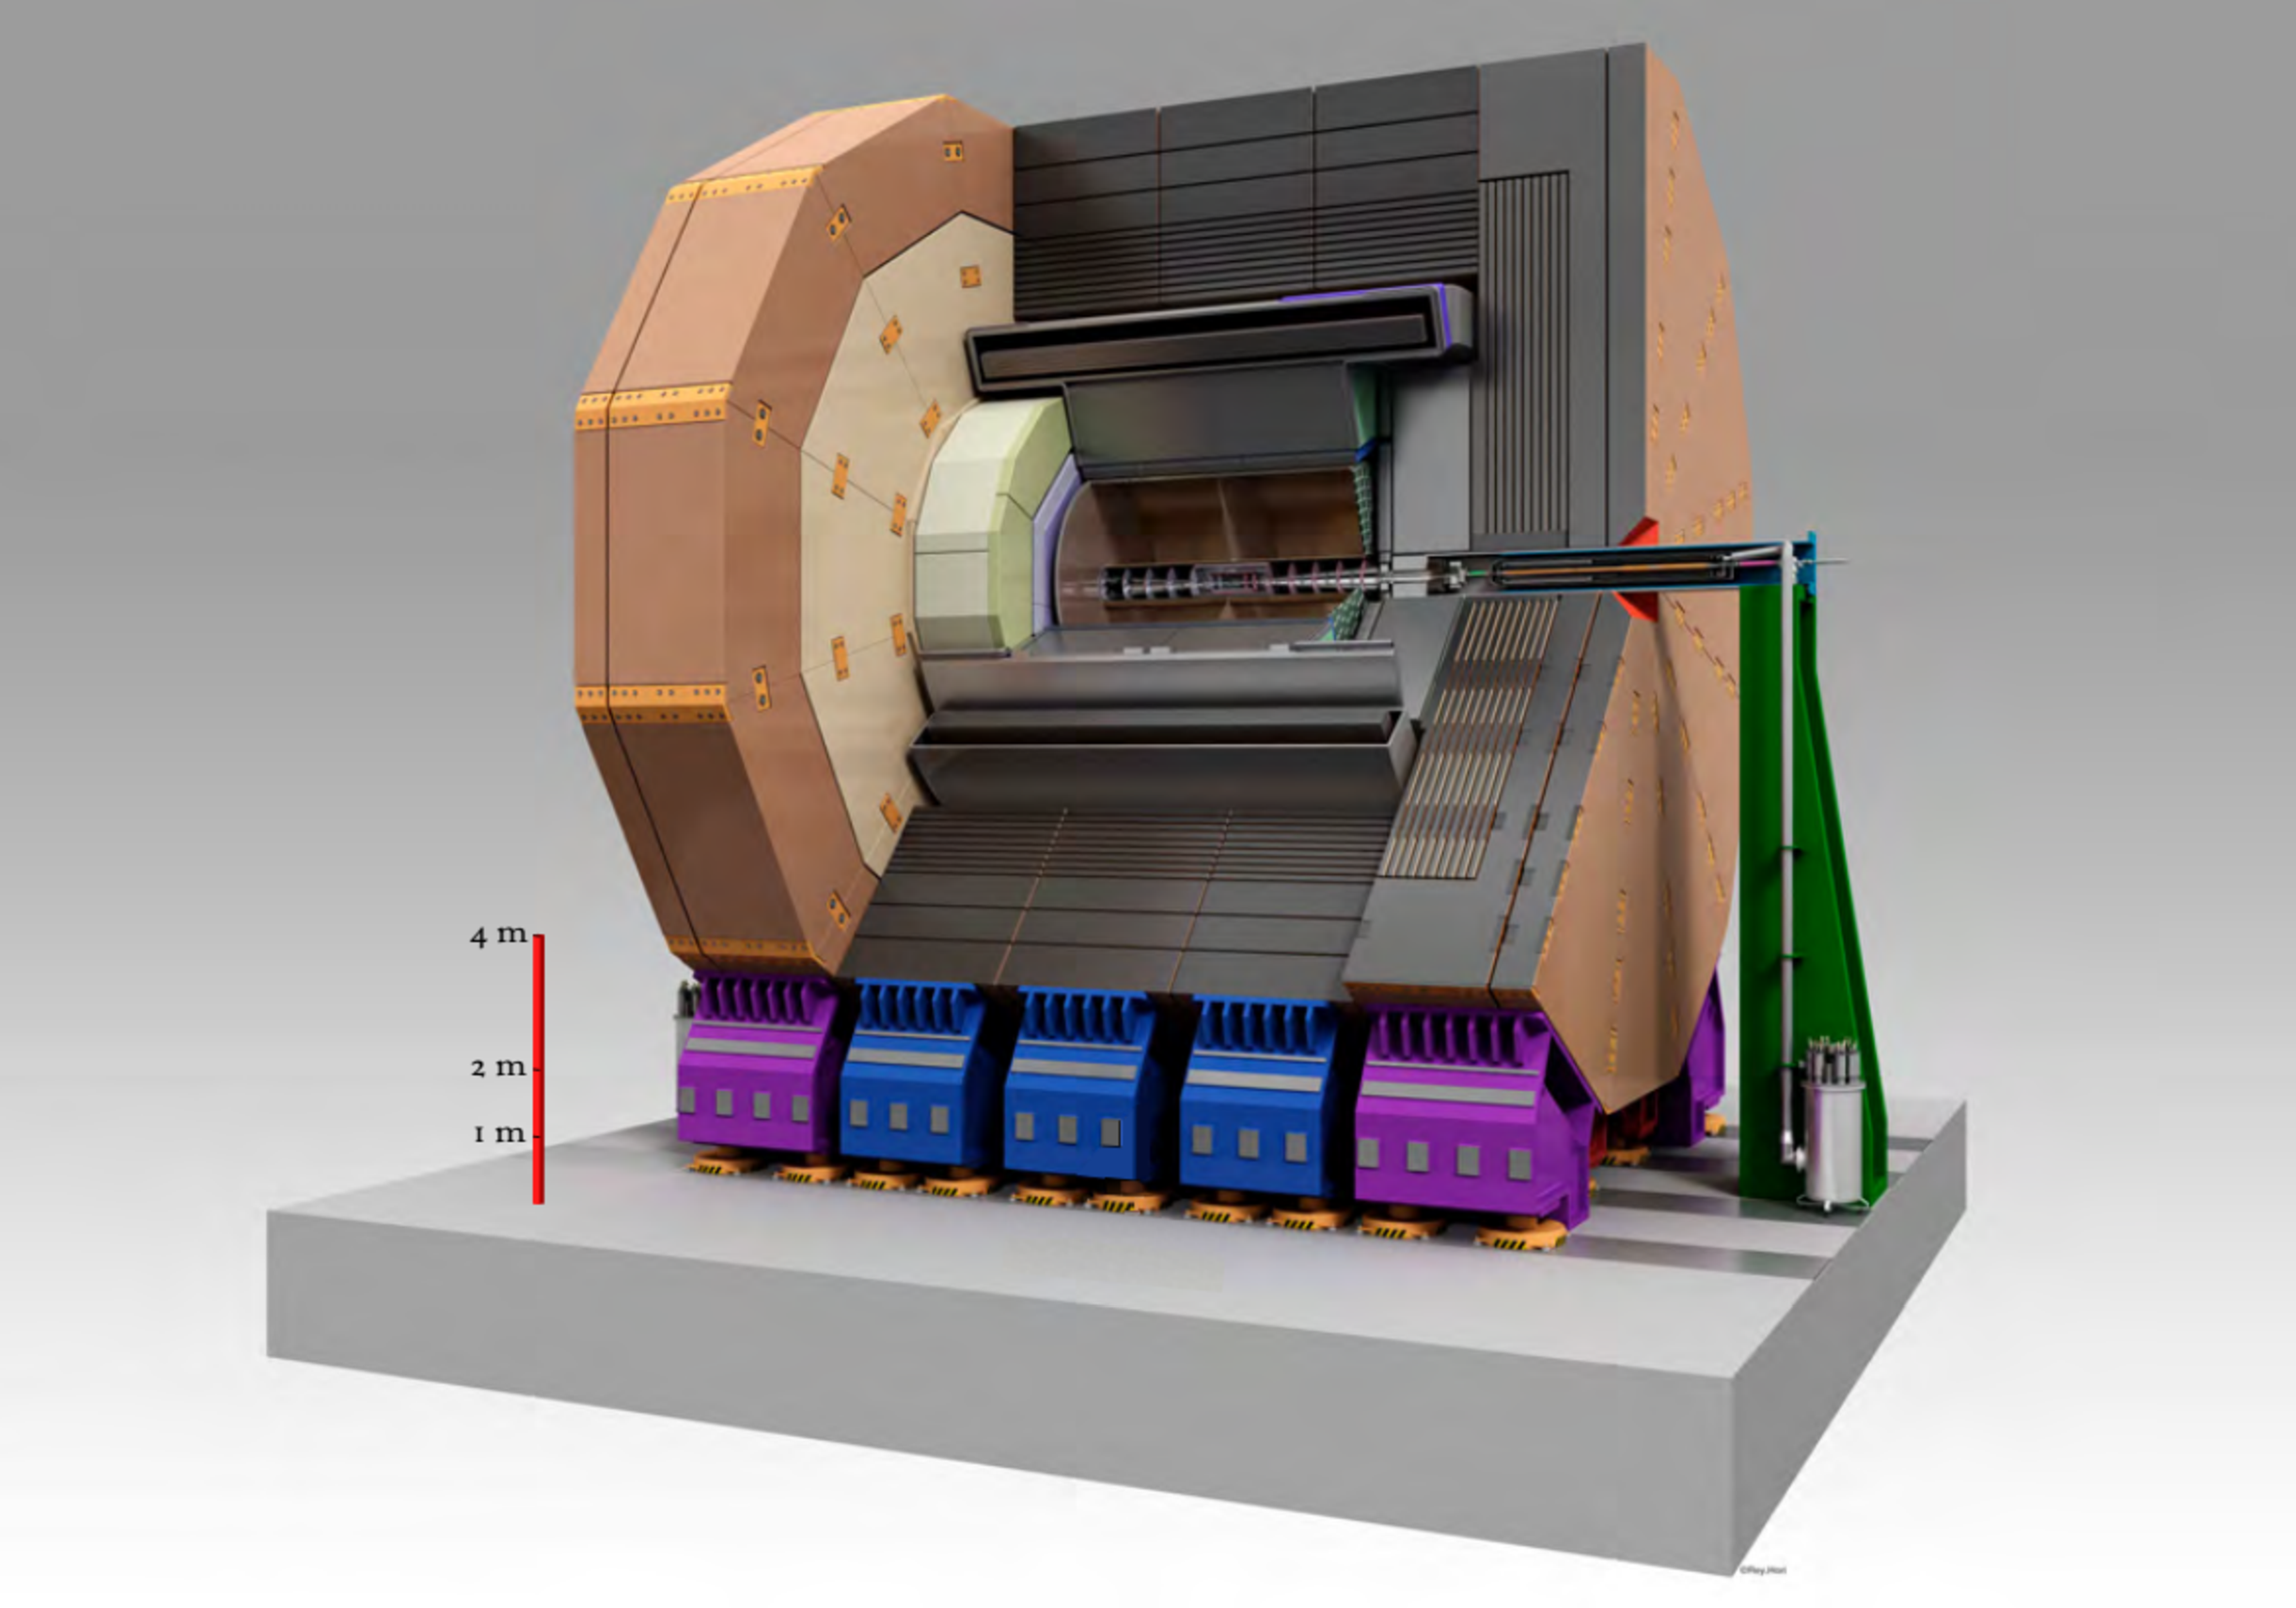
\includegraphics[scale=0.14]{ild3d.pdf}
\end{column}
\begin{column}{0.5\textwidth}
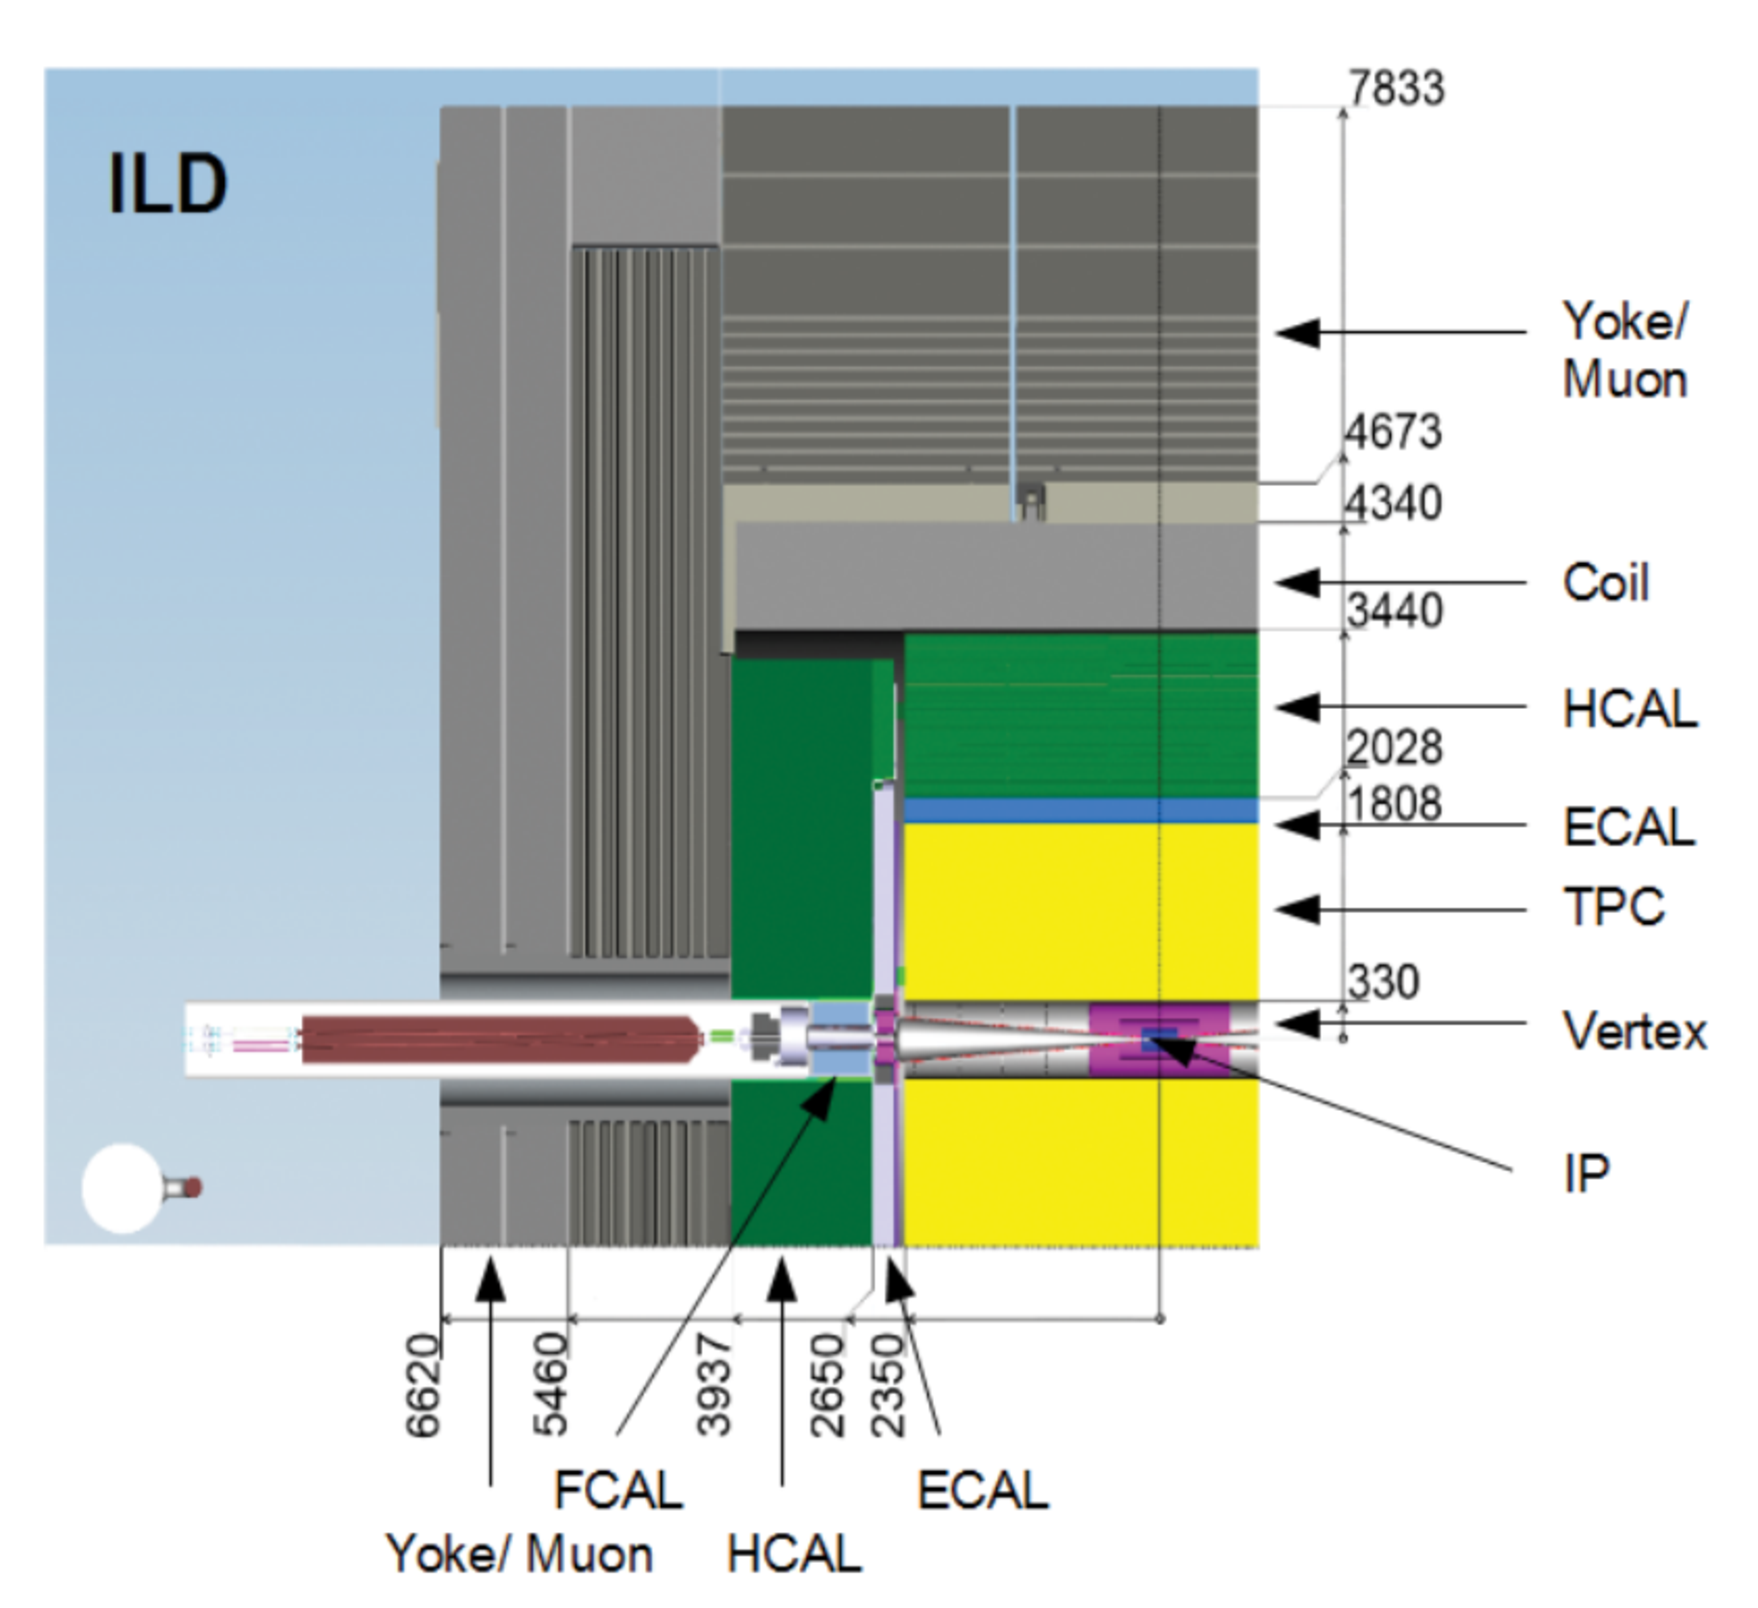
\includegraphics[scale=0.2]{ildxsec.pdf}
\end{column}
\end{columns}
\begin{itemize}
\item Maximizes detector particle resolving power by being large
\item 3.5T Magnetic Field
\item Gaseous Tracker $\rightarrow$ bubble chamber-like tracks
\end{itemize}
\end{frame}

\begin{frame}{Polarization primer }
A key feature of ILC is beam polarization\\
Use beams to control physics -- suppress or enhance certain processes which are sensitive to e/p helicity intital states\\
\quad \quad \\ 

Example beam scenario : $(P_{e^-}, P_{e^+}) = (-0.8,+0.3)$\\
$P_{e^\pm}$ is related to the fraction of Left or Right handed electron/positrons in a beam\\
\quad \quad \\

$P_{e^-} =-0.8$ means $e^-$ beam is $90\%$ L and $10\%$ R\\
$P_{e^+} =+0.3$ means $e^+$ beam is $65^\%$ R and $35\%$ L\\
\quad \quad\\

So.. in $(-0.8,+0.3)$\\
Most collisions will be between $e^-_L$ and $e^+_R$ (LR)\\
but sometimes the opposite occurs $e^-_R$ and $e^+_L$ (RL)\\
LL, RR is possible too (less important in WW) \\


\end{frame}

\begin{frame}{Introduction / Motivation}

\begin{columns}
\begin{column}{0.5\textwidth}
\feynmandiagram [horizontal=a to b] {
  i1 [particle=\(e^{-}\)] -- [fermion] a -- [fermion] i2 [particle=\(e^{+}\)],
  a -- [photon, edge label=\(\gamma / Z\)] b,
  f1 [particle=\(W^{+}\)] -- [photon] b -- [photon] f2 [particle=\(W^{-}\)],
};
    \feynmandiagram[vertical'=a to b ]{
        i1 [particle=\(e^{-}\)]
            -- [fermion] a 
            -- [boson] f1 [particle=\(W^{-}\)],
        a -- [fermion, edge label'=\(\nu\)] b ,
        i2 [particle=\(e^{+}\)]
            -- [anti fermion] b
            -- [boson] f2 [particle=\(W^{+}\)]
    };
\end{column}
\begin{column}{0.5\textwidth}
\begin{itemize}
	\item WW is a standard process with a large cross-section 
		
		
		\item Semileptonic mode offers significant advantages over fully hadronic/leptonic modes
\item Offers utility in both new physics potential and benchmarking detector performance
	\item Three central physics issues addressable by this channel are
		\begin{itemize}
		\scriptsize
		\item[--] Dynamics of the charged triple gauge couplings
		\item[--] Measurement of W boson mass, width, cross-section, and BR
		\item[--] Beam polarization measurement
		\end{itemize}
		\end{itemize}
\end{column}
\end{columns}

\end{frame}

\begin{frame}{500 GeV Samples}

Study here uses full simulation at $\sqrt{s} = 500$ GeV\\
Total luminosity : 4000 fb$^{-1}$\\
Polarizations:
\scriptsize
\begin{tabular}{|c|c|c|c|c|}
\hline 
Pol. &(-0.8,+0.3) & (+0.8,-0.3) & (-0.8,-0.3) & (+0.8,+0.3) \\ 
\hline 
Lum. [fb$^{-1}$] & 1600 & 1600 & 400 & 400 \\ 
\hline 
\end{tabular} 
\normalsize
\quad \quad \\
Reco/Sim: \quad \scriptsize
\url{ILCSoft v02-00-02} \quad
\url{ILD_l5_o1_v02}\\
\quad \quad \\
\normalsize
MC Background Samples (DBD)--\\

\begin{columns}
\begin{column}{0.5\textwidth}

\begin{itemize}

	\item[--] 2-fermion 
		\begin{itemize}
			\scriptsize
			\item[-] Z-bhabhag/hadronic/leptonic
		\end{itemize}
	\item[--] 4-fermion 
		\begin{itemize}
			\scriptsize
			\item[-] singleW-leptonic 
			\item[-]Zee/$\nu\nu$-leptonic/semileptonic 
			\item[-]singleZsingleWMix-leptonic 
			\item[-]WW-hadronic/leptonic
			\item[-]ZZ-hadronic/leptonic/semileptonic
			\item[-]ZZWWMix-hadronic/leptonic
		\end{itemize}
	

\end{itemize}

\end{column}
\begin{column}{0.5\textwidth}
\begin{itemize}
	\item[--] 6-fermion
	\begin{itemize}
		\scriptsize
		\item[-]eeWW, $\ell\ell$WW, $\nu\nu$WW, xxWW
		\item[-]ttbar
		\item[-]xxxxZ, yyyyZ
	\end{itemize}
	\item[--] SM Higgs
		\begin{itemize}
			\scriptsize
			\item[-] eeH, qqH, $\mu\mu$H, $\tau\tau$H, $\nu\nu$H
		\end{itemize}\quad\quad
\end{itemize}
\end{column}
\end{columns}


\end{frame}

\begin{frame}{Analysis Approach}
\textbf{Step 1}-\\
Treat all lepton flavors universally\\
Identify signal lepton candidates with TauFinder\\
\scriptsize
\begin{columns}
\begin{column}{0.5\textwidth}
\begin{itemize}
\item Optimize TauFinder to efficiently find lepton jets based on decay signatures
\item Simultaneously reject fake lepton jets from hadronic jets
\item Examine 7 separate categories of lepton jets
\end{itemize}
\end{column}
\begin{column}{0.5\textwidth}

		Optimization Categories:\\
		\quad \quad \\
		Prompt $\mu$\\
		Prompt $e$\\
		Inclusive $\tau$\\
		$\tau\rightarrow \mu \nu_{\mu} \nu_{\tau}$ \\
		$\tau\rightarrow e \nu_{e} \nu_{\tau}$\\
		$\tau \rightarrow$ hadronic (1-prong)\\
		$\tau \rightarrow$ hadronic (3-prong)\\

\end{column}
\end{columns}
\quad \quad \quad 
\\	%This approach simultaneously optimizes lepton selection for prompt $\mu/e$\\
	\normalsize
\textbf{Step 2}-\\
With a selected lepton, treat the remaining system as hadronic components of $W\rightarrow qq$\\
\quad \quad \scriptsize Use y-cut and kinematic cuts on mini-jets to mitigate pileup ($\gamma \gamma$)\\
\normalsize
\textbf{Step 3}- Perform basic event selection for most favorable polarization scenario\\
\textbf{Step 4}- Obtain physics measurements\\
\end{frame}

\begin{frame}{(1) TauFinder}
\textbf{TauFinder basic operation}\\
\begin{itemize}
\item Seed lepton jet candidates with tracks ordered by $|P|$\\
\item All particles within the search cone are added to the lepton jet\\
\item Each candidate is subjected to acceptance conditions \\
\end{itemize}
\quad \quad \\
\begin{columns}
\begin{column}{0.5\textwidth}
\scriptsize \textbf{Operating Criteria/Acceptance Conditions}
 \begin{itemize}
 \scriptsize
 	\item[-]\textbf{Search Cone Angle} \colorbox{orange}{$\alpha$}- The opening angle of the search cone for the lepton jet [rad]
 	\item[-] \textbf{Isolation Cone Angle} \colorbox{red}{$\beta$} - Outer isolation cone around the search cone of the lepton jet [rad]
 	\item[-] \colorbox{lightblue}{\textbf{Isolation Energy}} - The total energy allowed within the isolation cone region [GeV]
 	\item[-]Invariant Mass - The upper limit on lepton candidate mass [GeV]
 	\item[-] $0 <$ Max N Tracks $\leq 3$
 \end{itemize}
\end{column}
\begin{column}{0.5\textwidth}
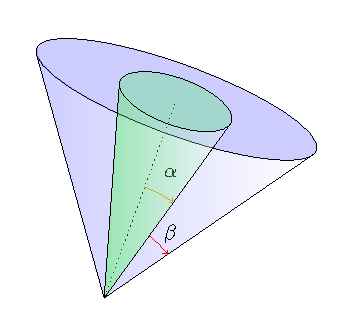
\includegraphics[scale=0.7]{cone.pdf}
\end{column}
\end{columns} 
 
\end{frame}

\begin{frame}{(1) TauFinder Optimization}
\begin{columns}
\begin{column}{0.5\textwidth}
Optimization of 3 parameters $\alpha \, , \beta \, , E_{iso}$\\
Fixed Mass $\leq 2$ GeV

\end{column}
\begin{column}{0.5\textwidth}
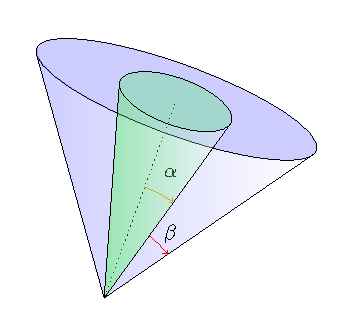
\includegraphics[scale=0.6]{cone.pdf}
\end{column}
\end{columns}


\begin{columns}
\begin{column}{0.5\textwidth}
Maximize \textbf{Efficiency for true leptons} \\
\scriptsize using $WW\rightarrow qq \ell \nu$ 
\\
\colorbox{yellow}{$\varepsilon_s = N_{matched}/N_{Stotal} $}\\
	\scriptsize
	\begin{itemize}
	\item[-] $N_{matched} \geq$ 1 candidate matched within 100 mrads of the Gen. lepton/visible components\\ 
	\item[-] $N_{Stotal}$ includes an acceptance cut with 3 visible Gen. fermions $|cos\theta |< 0.99$
	\end{itemize}
	\normalsize	
	Optimal working point at:\\
	\quad \quad \quad \colorbox{green}{ max$[(1-P_{fake}) \varepsilon_s]$}
\end{column}
\begin{column}{0.5\textwidth}
Minimize
\textbf{Probability of fake leptons}\\
\scriptsize using $WW \rightarrow qqqq$ \\
\colorbox{yellow}{$P_{fake} = 1-(1 - \varepsilon_b)^{\frac{1}{4} }$}\\

\colorbox{yellow}{ $\varepsilon_b = N_b/N_{Btotal}$} \\
	\scriptsize
	\begin{itemize}
	\item[-] $P_{fake} =$ probability of 1 success(fake) given 1 trial(jet)\\
	\item[-] $N_b \geq$ 1 reconstructed lepton jet from all 4 jets\\
	\item[-] $N_{Btotal}$ includes an acceptance cut with 4 visible Gen. fermions $|cos\theta |< 0.99$
	\end{itemize}

\end{column}
\end{columns}

\end{frame}

\begin{frame}{(1) TauFinder Optimization Results}
\scriptsize
Optimized against $qq\ell \nu$ and $qqqq$ samples with $100\% \, \, e^-_L e^+_R$ polarization 

\tiny
\begin{tabular}{|p{0.1\textwidth}|p{0.13\textwidth}p{0.13\textwidth}p{0.13\textwidth}p{0.1\textwidth}p{0.1\textwidth}p{0.1\textwidth}|}

\hline 
\rowcolor{lightgray}
Channel & $n \, \, \text{Lep} \geq 1$ & $1-P_{F}$ & $\epsilon_T$ & SearchCone [rad] & Iso.Cone [rad] & Iso.E [GeV] \\ 
\hline 
\rowcolor{green}
Prompt $\mu$ & $0.955 \pm 0.003$ & $0.974 \pm 0.001$ & $0.949 \pm 0.003$ & 0.03 & 0.15 & 3.0 \\ 

Prompt $e$ & $0.920 \pm 0.003$ & $0.961 \pm 0.001$ & $0.904 \pm 0.003$ & 0.04 & 0.15 & 4.0 \\ 
\rowcolor{emerald}
Inclusive $\tau$ & $0.800 \pm 0.005$ & $0.943 \pm 0.001$ &  $0.770 \pm 0.006$ & 0.07 & 0.15 & 4.5 \\ 


 \hline
$\tau \rightarrow \nu \nu \mu$ & $0.815 \pm 0.012$ & $0.974 \pm 0.001$ & $0.801 \pm 0.013$ & 0.03 & 0.15 & 3.0 \\ 
 
$\tau \rightarrow \nu \nu e$ &  $0.800 \pm 0.012$ & $0.963 \pm 0.001$ &  $0.781 \pm 0.013$ & 0.05 & 0.15 & 3.5 \\ 
 
$\tau$ Had-1p & $0.744 \pm 0.009$ & $0.930 \pm 0.002$ & $0.707 \pm 0.009$ & 0.07 & 0.15 & 4.5 \\ 
 
$\tau$ Had-3p &  $0.756 \pm 0.015$ & $0.930 \pm 0.002$ & $0.710 \pm 0.016$ & 0.07 & 0.15 & 5.5  \\
\hline
\end{tabular} 
\quad \quad \\
\quad \quad \\
\begin{itemize}
\scriptsize
\item Trickier reconstruction suggests wider cones and more isolation energy
\item Use two cones for analysis \colorbox{green}{Prompt $\mu$} and \colorbox{emerald}{Inclusive $\tau$} for a \colorbox{green}{Tight} and \colorbox{emerald}{Loose} selection
\item Expect tight selection to best capture all high quality lepton candidates
\item Loose selection should boost efficiency of hadronic $\tau$
\end{itemize}




\end{frame}

\begin{frame}{(2) Hadronic System}

\begin{columns}
\begin{column}{0.5\textwidth}
If a lepton has been found, 
\begin{itemize}
\scriptsize
\item[-]select highest energy candidate as signal lepton\\
\item[-] shuffle remaining fakes back into the hadronic system.\\
\end{itemize}
\scriptsize
At least one quark tends to be very forward, so pileup tends to mix into the jets\\
\quad \quad \\
These beam particles cannot be cleanly removed by standard methods e.g. kT algorithm with tuned R values\\

\end{column}
\begin{column}{0.5\textwidth}

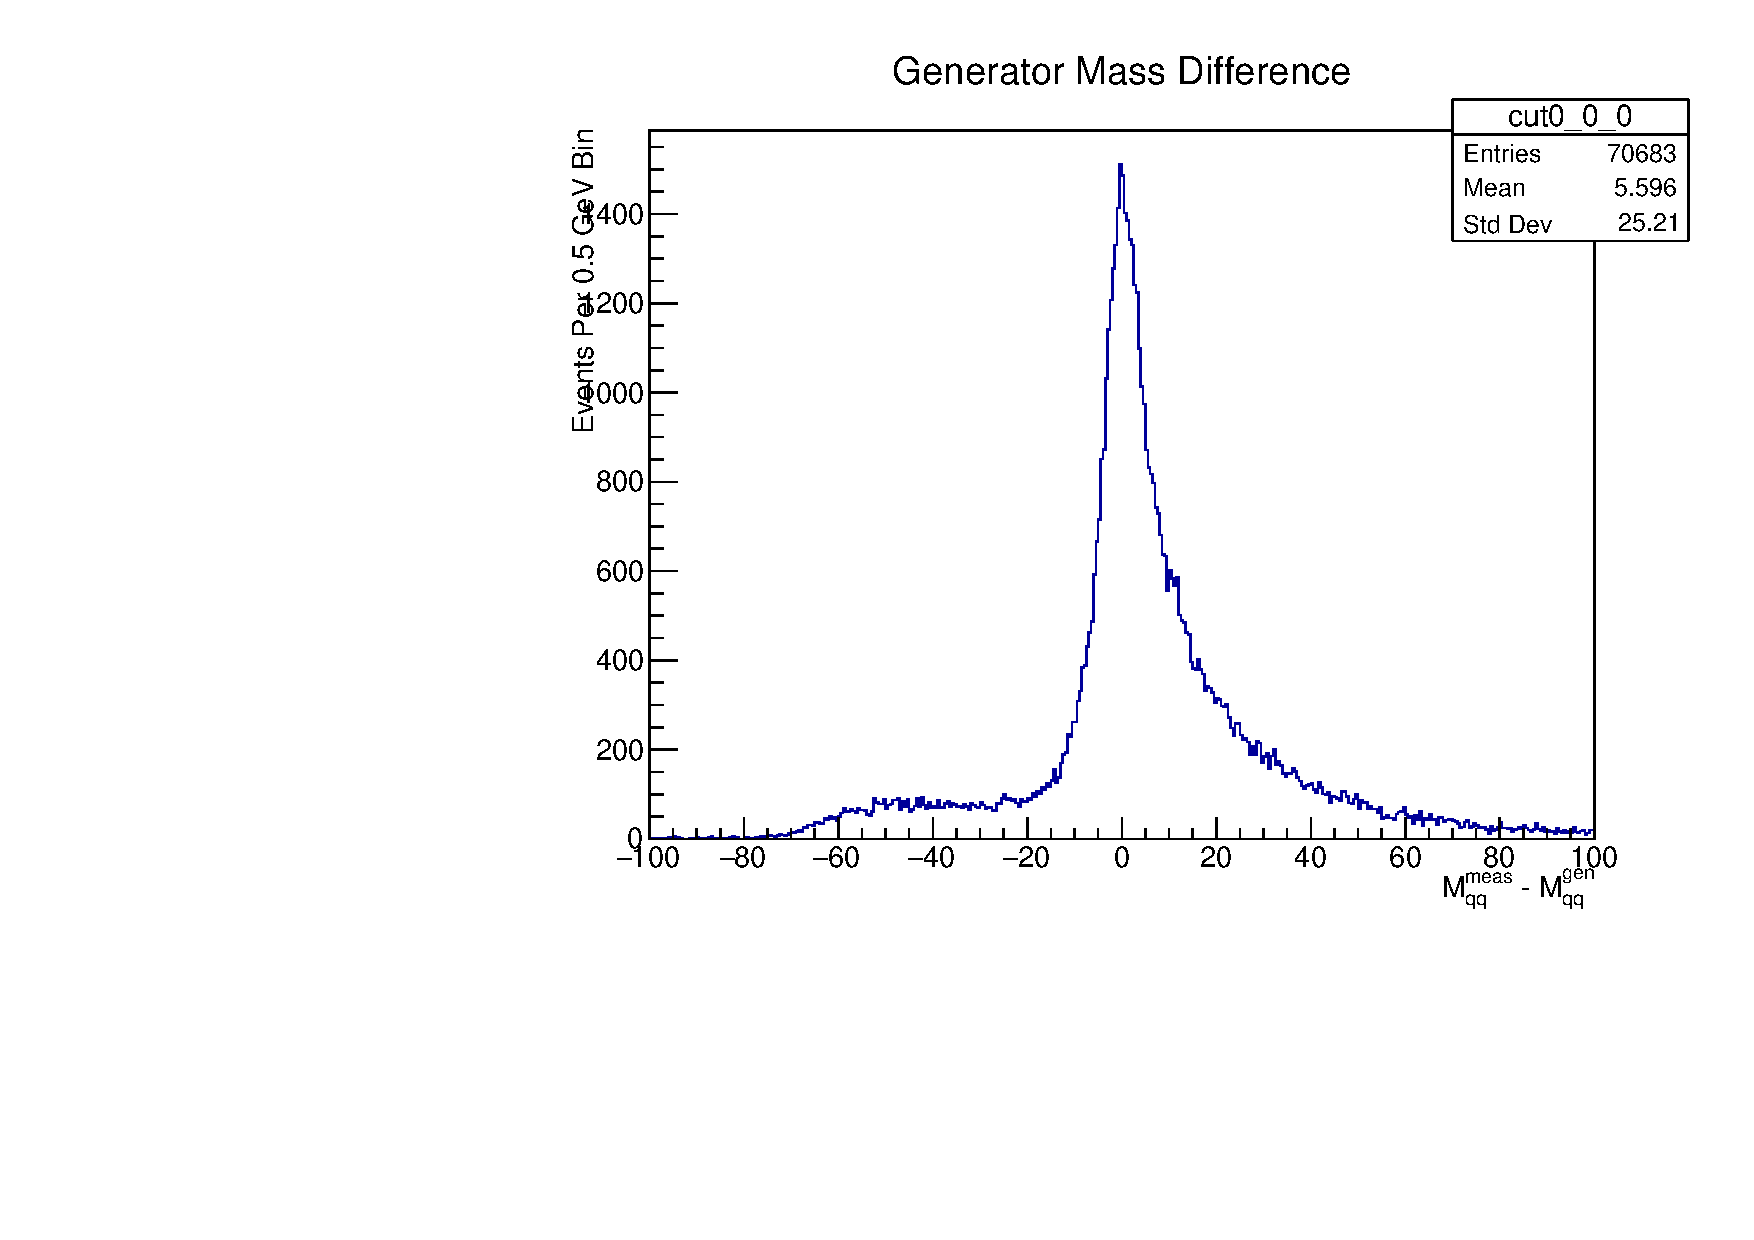
\includegraphics[scale=0.3]{nocutDiff.pdf}\\
\scriptsize
\quad $100\% \, \, e^-_L e^+_R$ polarization\\
 Measured mass is often larger than the true value \\



\end{column}
\end{columns}
\normalsize
Mitigate Pileup with ``Jet Fragmentation"\\
  \begin{itemize}
  	\scriptsize
  \item[-]tune y-cut($\propto M^2_{jet}$) values on the durham algorthim (eekt)
  \item[-]apply simple cuts to the resulting ``mini-jets"\\
  \end{itemize}

\end{frame}
\begin{frame}{(2) Optimized W Mass}
\begin{columns}
\begin{column}{0.5\textwidth}
Find best y-cut combined with kinematic cuts to optimize hadronic W mass\

\quad \quad \\
Use 2 optimization parameters from the $M_{qq}^{meas} - M_{qq}^{gen}$ dist.:\\
\begin{itemize}
\item[-]Minimize Full Width Half Maximum (FWHM) \\
\item[-]Maximize Number of bin Entries in the Mode\\
\end{itemize}
\end{column}
\begin{column}{0.5\textwidth}
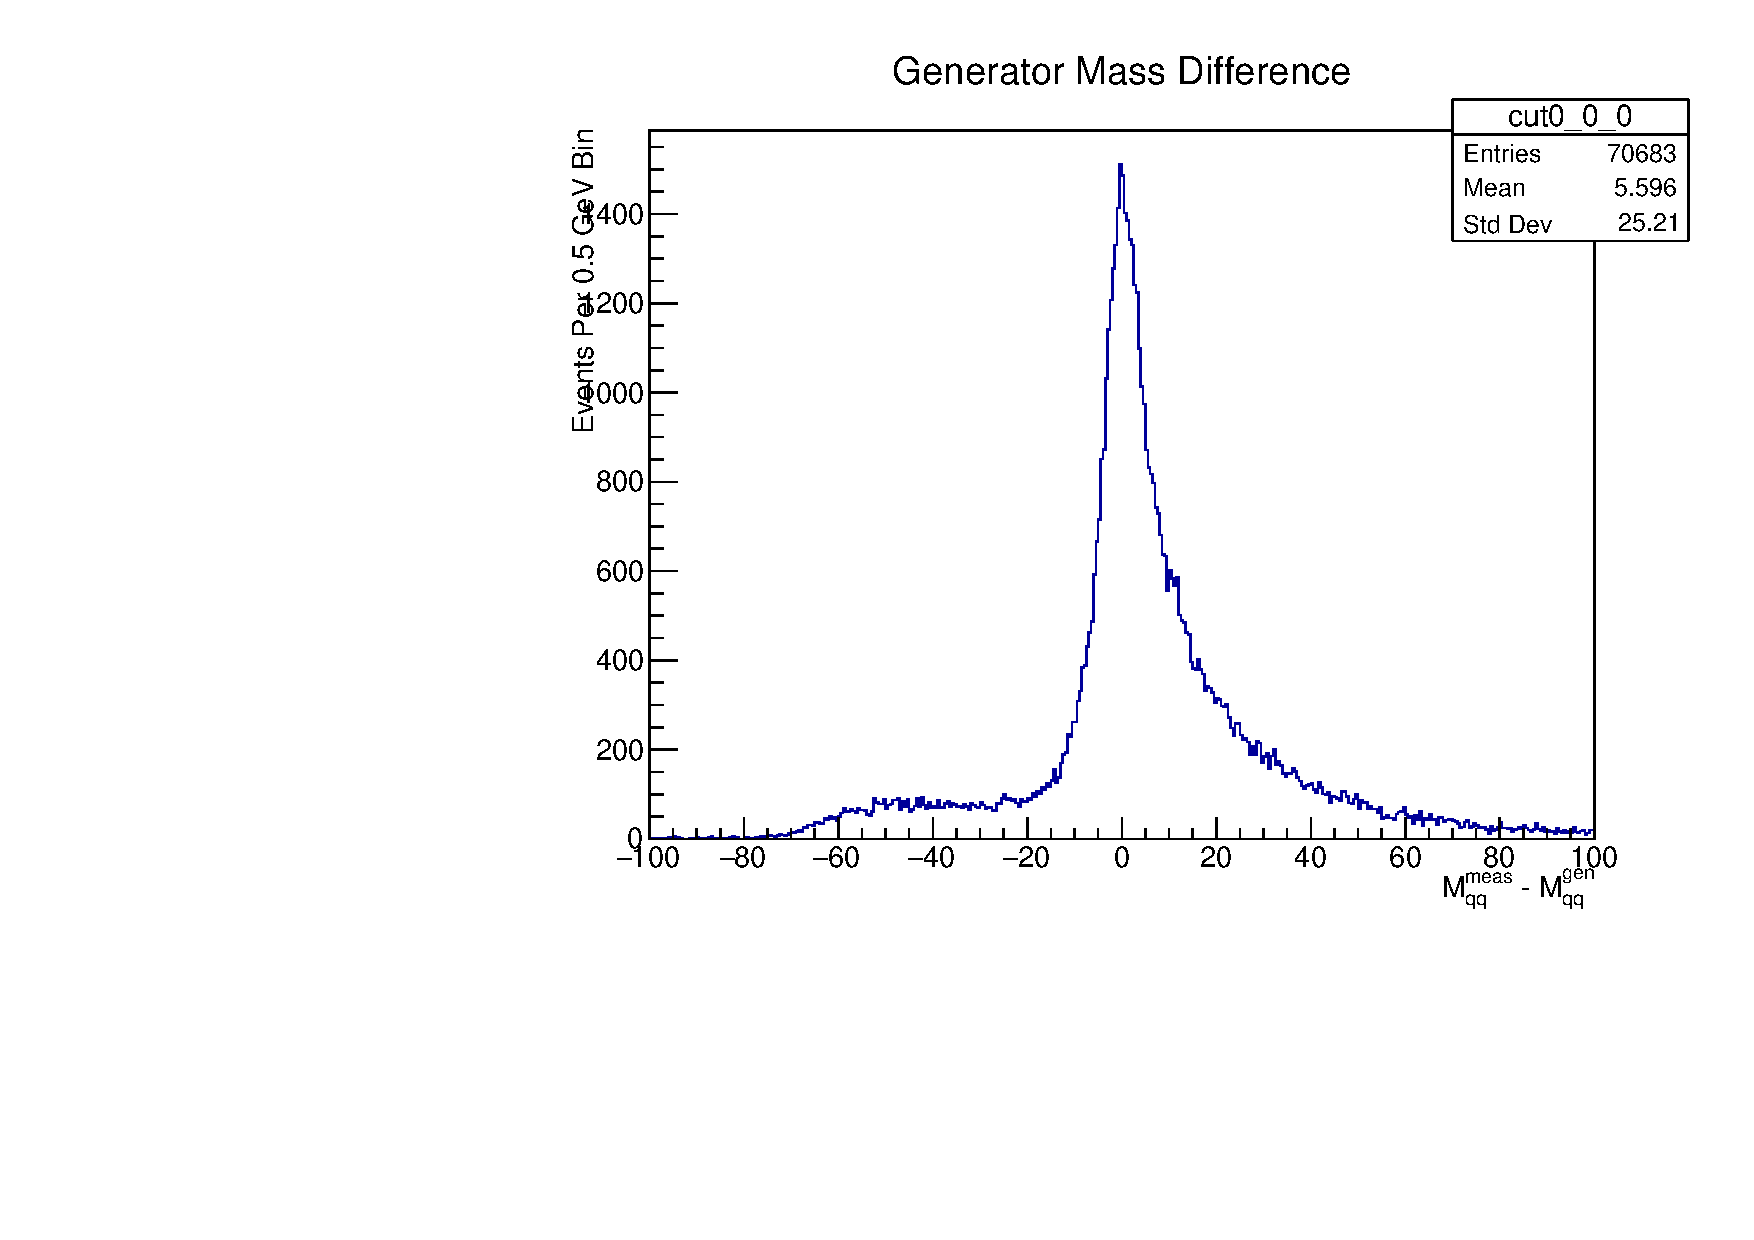
\includegraphics[scale=0.3]{nocutDiff.pdf}\\
\end{column}
\end{columns}
\quad \quad \\ 
\scriptsize
The Mode Entries is the number of entries in the Maximum bin + the number of Entries of the nearest left/right neighbor bins\\
The Mode is the weighted mean of the center of the 3 Mode bins\\
\quad \quad \\ 
The Maximum for the FWHM is the "Mode Average" or the average number of entries from the 3 mode bins\\
\quad \quad \\ 
The edges of the Width for FWHM are the weighted average between the 2 bins around the half maximum ( 1 bin above 1 bin below) 
\end{frame}

\begin{frame}{(2) Hadronic System Results}

\begin{columns}
\begin{column}{0.5\textwidth}
   	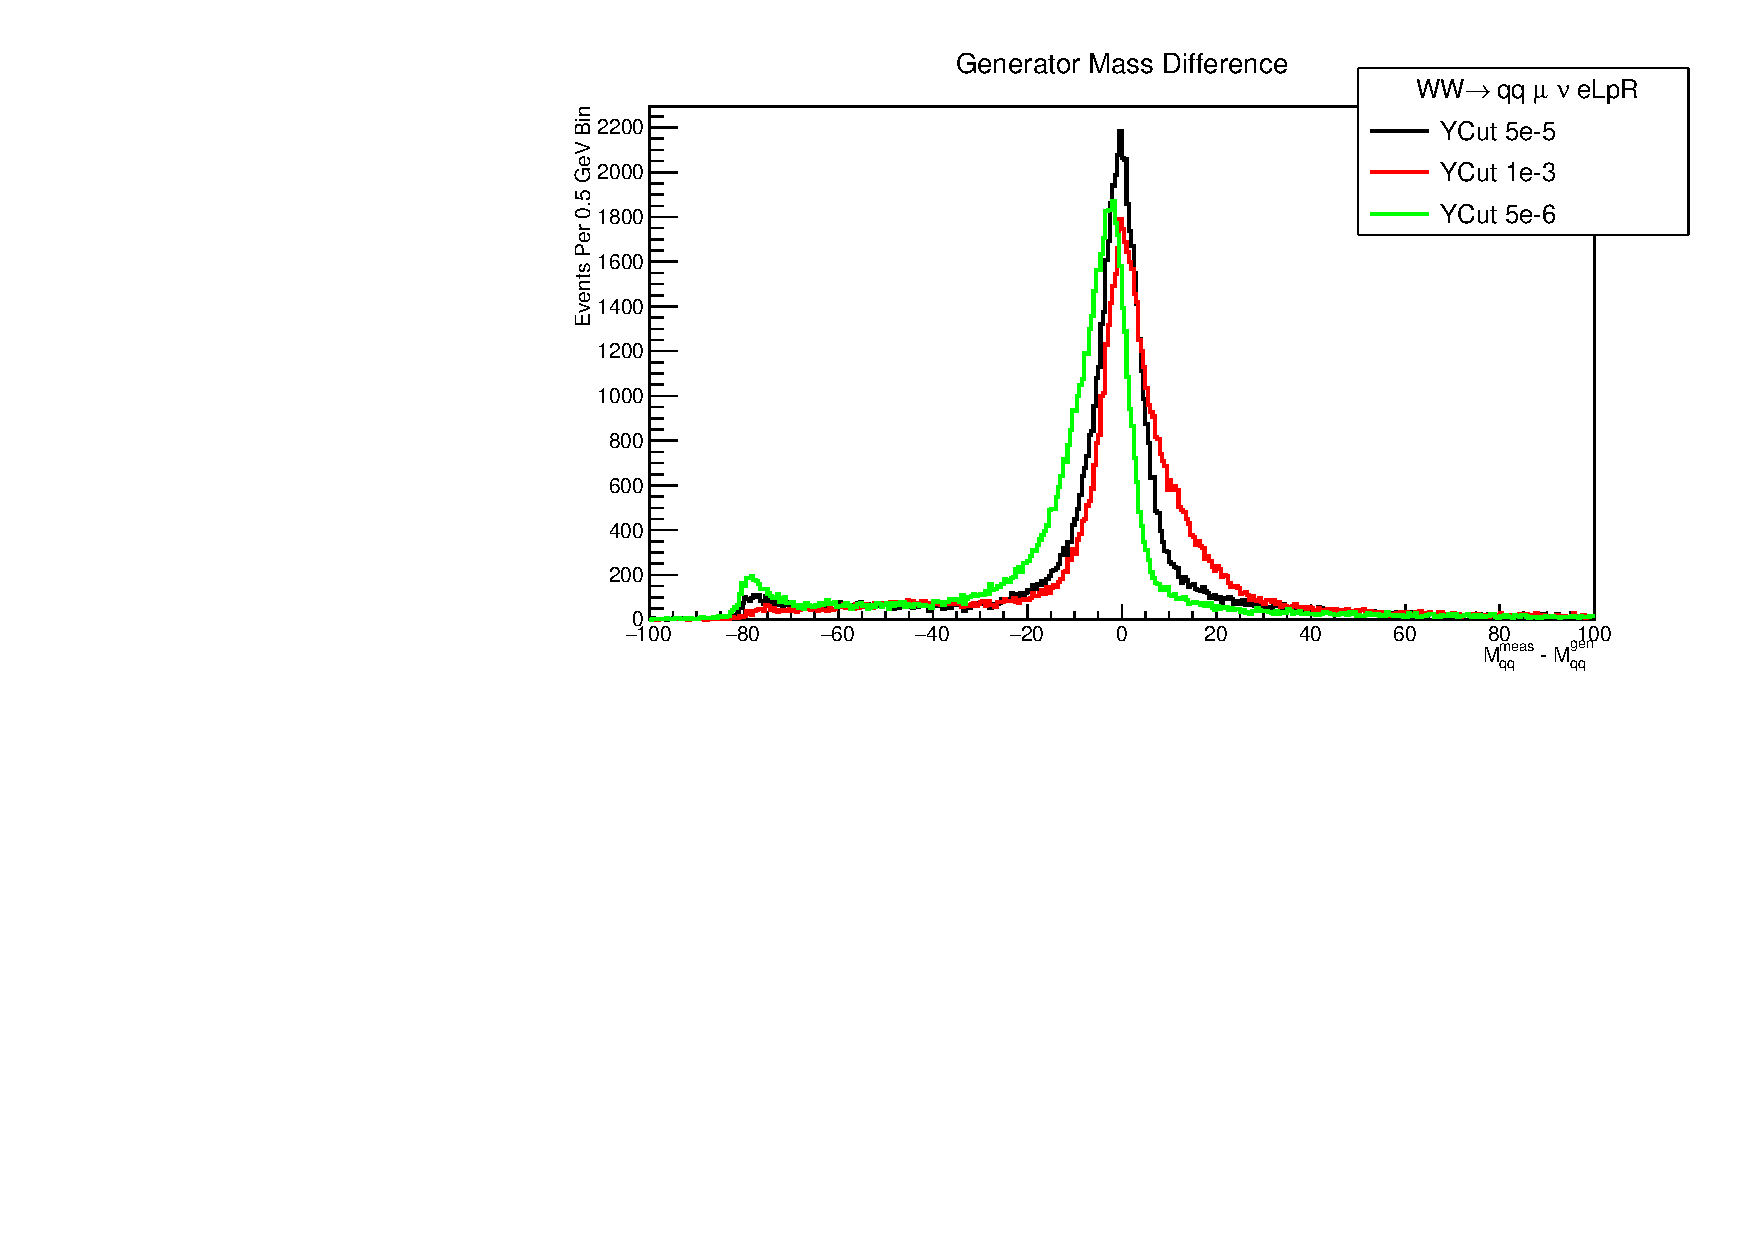
\includegraphics[scale=0.3, left]{SupDiff.pdf}\\
   	\scriptsize
   	Comparison of 3 YCuts with the same kinematic cuts Pt$>$2 GeV AND $|cos\theta|<$1 (optimized for 5e-05)\\
   	\quad \quad \\
   	Small peak around -80 GeV is where the W has been incorrectly thrown out\\
   	\quad \quad \\
   	
   
\end{column}
\begin{column}{0.5\textwidth}
	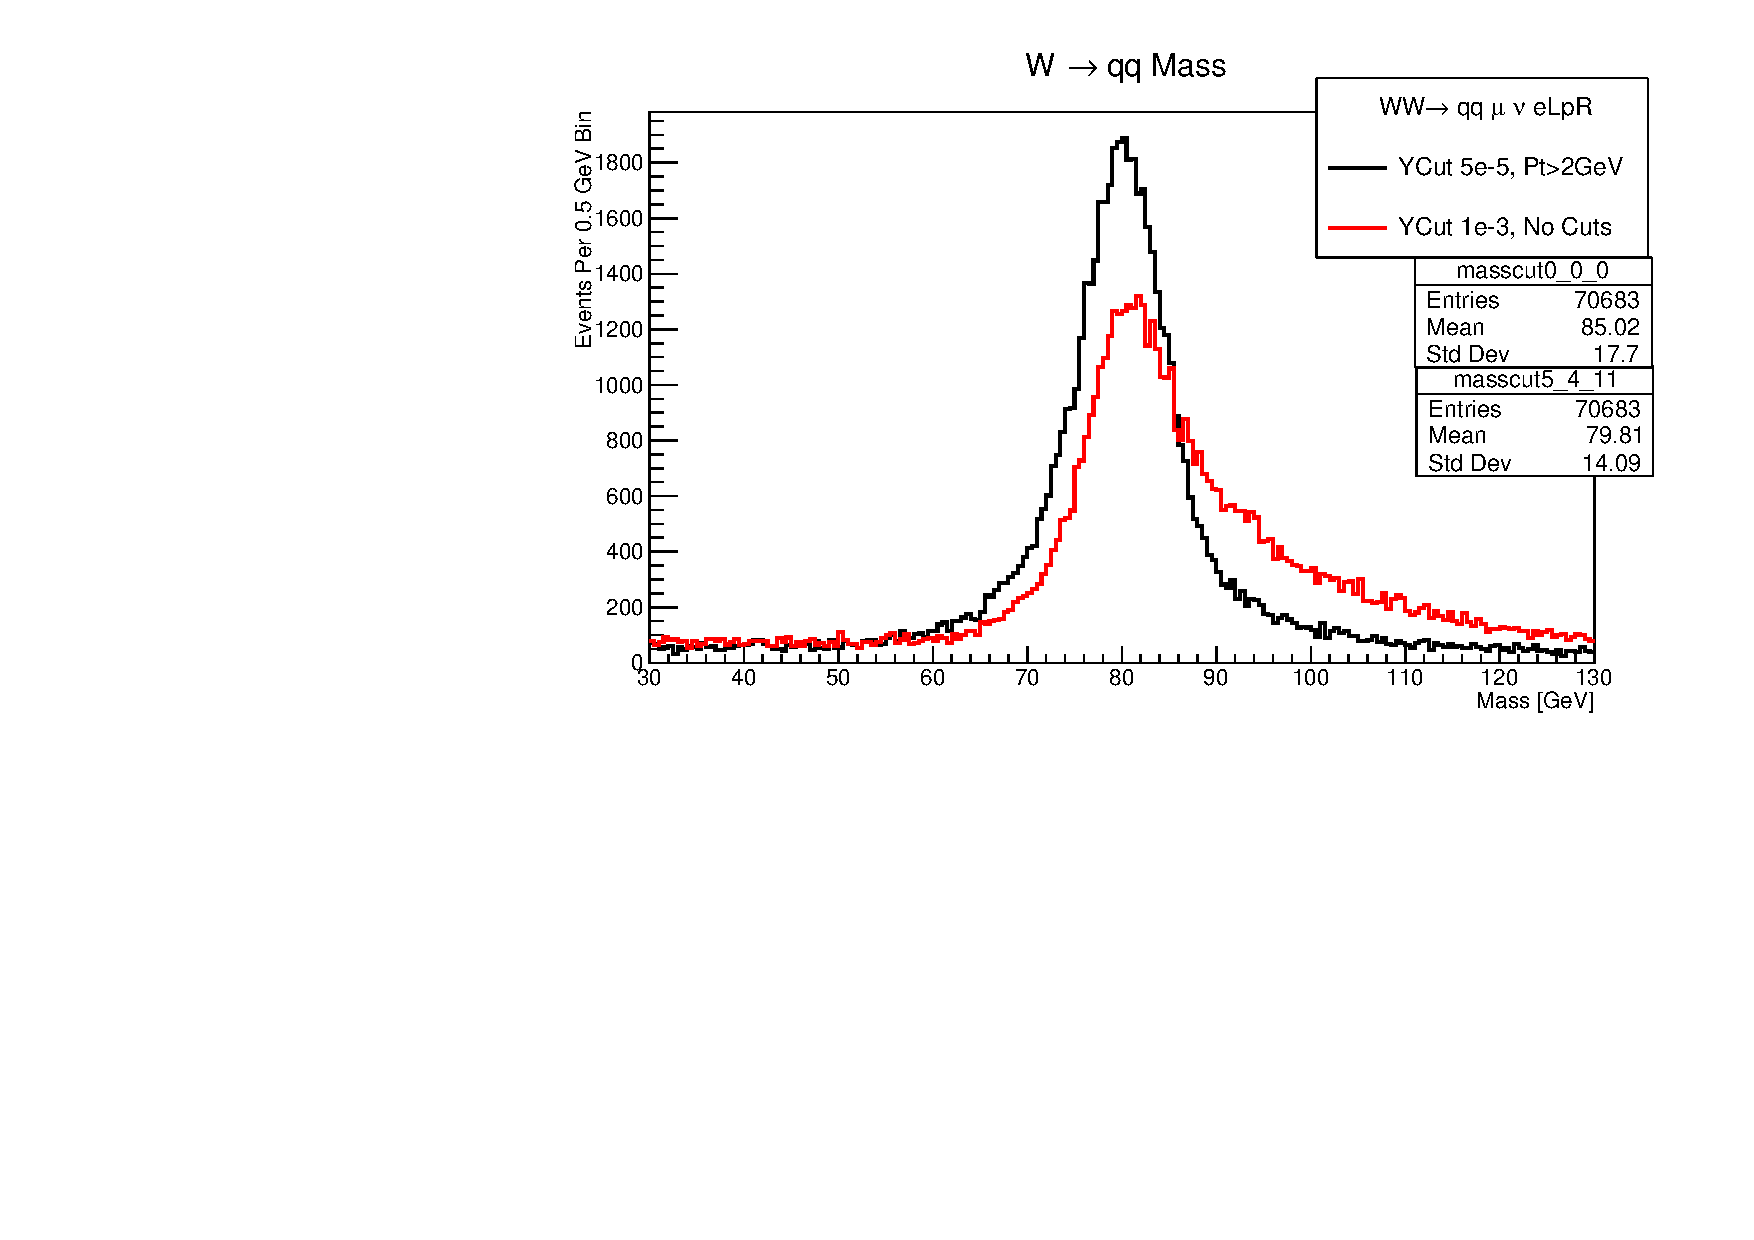
\includegraphics[scale=0.3, left]{SupMass.pdf}\\
	\scriptsize
	\quad \quad \quad \quad Significant Improvement !
\end{column}	
\end{columns}
\tiny
 Mass Difference Statistics:\\
 ycut: 0.001  ptcut: 2  costcut: 1  FWHM: 11.769 RMS: 24.1855 Mode: -0.24211 mean: 0.782898 modeEnt: 5199\\
 ycut: 5e-05  ptcut: 2  costcut: 1  FWHM: 9.7087 RMS: 25.2774 Mode: -0.25127 mean: -3.09776 modeEnt: 6326\\
 ycut: 5e-06  ptcut: 2  costcut: 1  FWHM: 11.567 RMS: 25.7475 Mode: -1.75521 mean: -9.57673 modeEnt: 5475\\

\quad \quad \\
\normalsize
Best Performance is reached with:\\
\textbf{ycut= 5e-05 and removal of mini-jets with pT $<$ 2 GeV }


\end{frame}
\begin{frame}{(3) Event Selection Overview}
Perform event selection with two mutually exclusive groups:\\
1st group will use $\mu$ cone (optimized for prompt muons)
	\begin{itemize}
		\scriptsize
		\item[-]\colorbox{green}{Tight} selection will yield some \colorbox{green}{efficiency $\epsilon_0$ and purity $p_0$}
		\item[-] tight cuts will be targeted towards prompt signal leptons $\mu/e$ 
	\end{itemize} 
2nd group will use the $\tau$ cone (optimized for inclusive $\tau$ decays)
	\begin{itemize}
	\scriptsize
		\item[-] \colorbox{emerald}{Loose} selection will yield some \colorbox{emerald}{efficiency $\epsilon_1$ and purity $p_1$}
		\item[-] Loose cuts should address $\tau$s not reconstructed by muon cone
		\item[-] orthogonalize selection require 0 tight leptons in loose selection
	\end{itemize}
Overall efficiency \colorbox{yellow}{$\epsilon = \epsilon_0 + \epsilon_1$}\\
Overall purity \colorbox{yellow}{$p = (N_0 + N_1) / (B_0 + B_1 + N_0 +N_1)$}\\
\quad \quad \\
Selection is optimized to maximize $\epsilon \cdot p$ for the subset of events where both fermion pairs are near the nominal W-mass

\end{frame}
\begin{frame}
Description of current cuts:(currently tight/loose are mostly the same)\\
\tiny
adapted from ref. \url{I. Marchesini DESY-THESIS 2011}\\
\scriptsize
--Note reconstucted particles are boosted against crossing angle boost-- (3.5 GeV in x)\\
\begin{itemize}
\item[-]\colorbox{orange}{Lepton} - Require at least 1 reconstructed lepton
\item[-]\colorbox{orange}{Track Multiplicity $> 10$} - more than 10 tracks in the event (Before pileup removal)
\item[-]\colorbox{orange}{Pt $> 5$ GeV} - Reject events with no genuine missing Pt 
\item[-]\colorbox{orange}{$E_{vis} < 500$ GeV} Sum of the total visible energy in the event 
\item[-]\colorbox{orange}{$E_{com} > 100$ GeV} - Rest-frame energy with visible and inferred missing energy\\  \quad $E_{com} = E_{vis} + |P_{miss}| \, \,  \, \text{and} \, \, P^\mu_{miss} = (|P_{miss}| , -\sum{\vec{p}_{vis}}) $
\item[-]\colorbox{orange}{$40<M_{qq}<120$} - constrains hadronic system to be W-like
\item[-]\colorbox{orange}{ $-qcos\theta_W$} - limit the $W^-$ backward scattering
\item[-]\colorbox{orange}{ $m^2_{\nu recoil} < 135,000 \, \, \text{GeV}^2$} - Require the visible system to recoil against a low mass object \\
\quad $m^2_{\nu recoil} = s + M^2_{vis} - 2\sqrt{s}E_{vis} \, \, \text{and} \, \, M^2_{vis} = ( P^{\mu}_{qq} +  P^{\mu}_{\ell})^2$ 

\end{itemize}
\end{frame}

\begin{frame}{(3) Event Selection (Tight)}

Example of the most powerful cuts:\\
\scriptsize
Tight Signal $\Rightarrow$  muon cone for $\mu,e,\tau$ signal events\\
All plots include an N Lepton $> 0$ cut \\
Polarization: (-0.8,+0.3)\quad
Luminosity: 1600 fb$^{-1}$
(Includes off-shell types of events)
\begin{columns}
\begin{column}{0.5\textwidth}
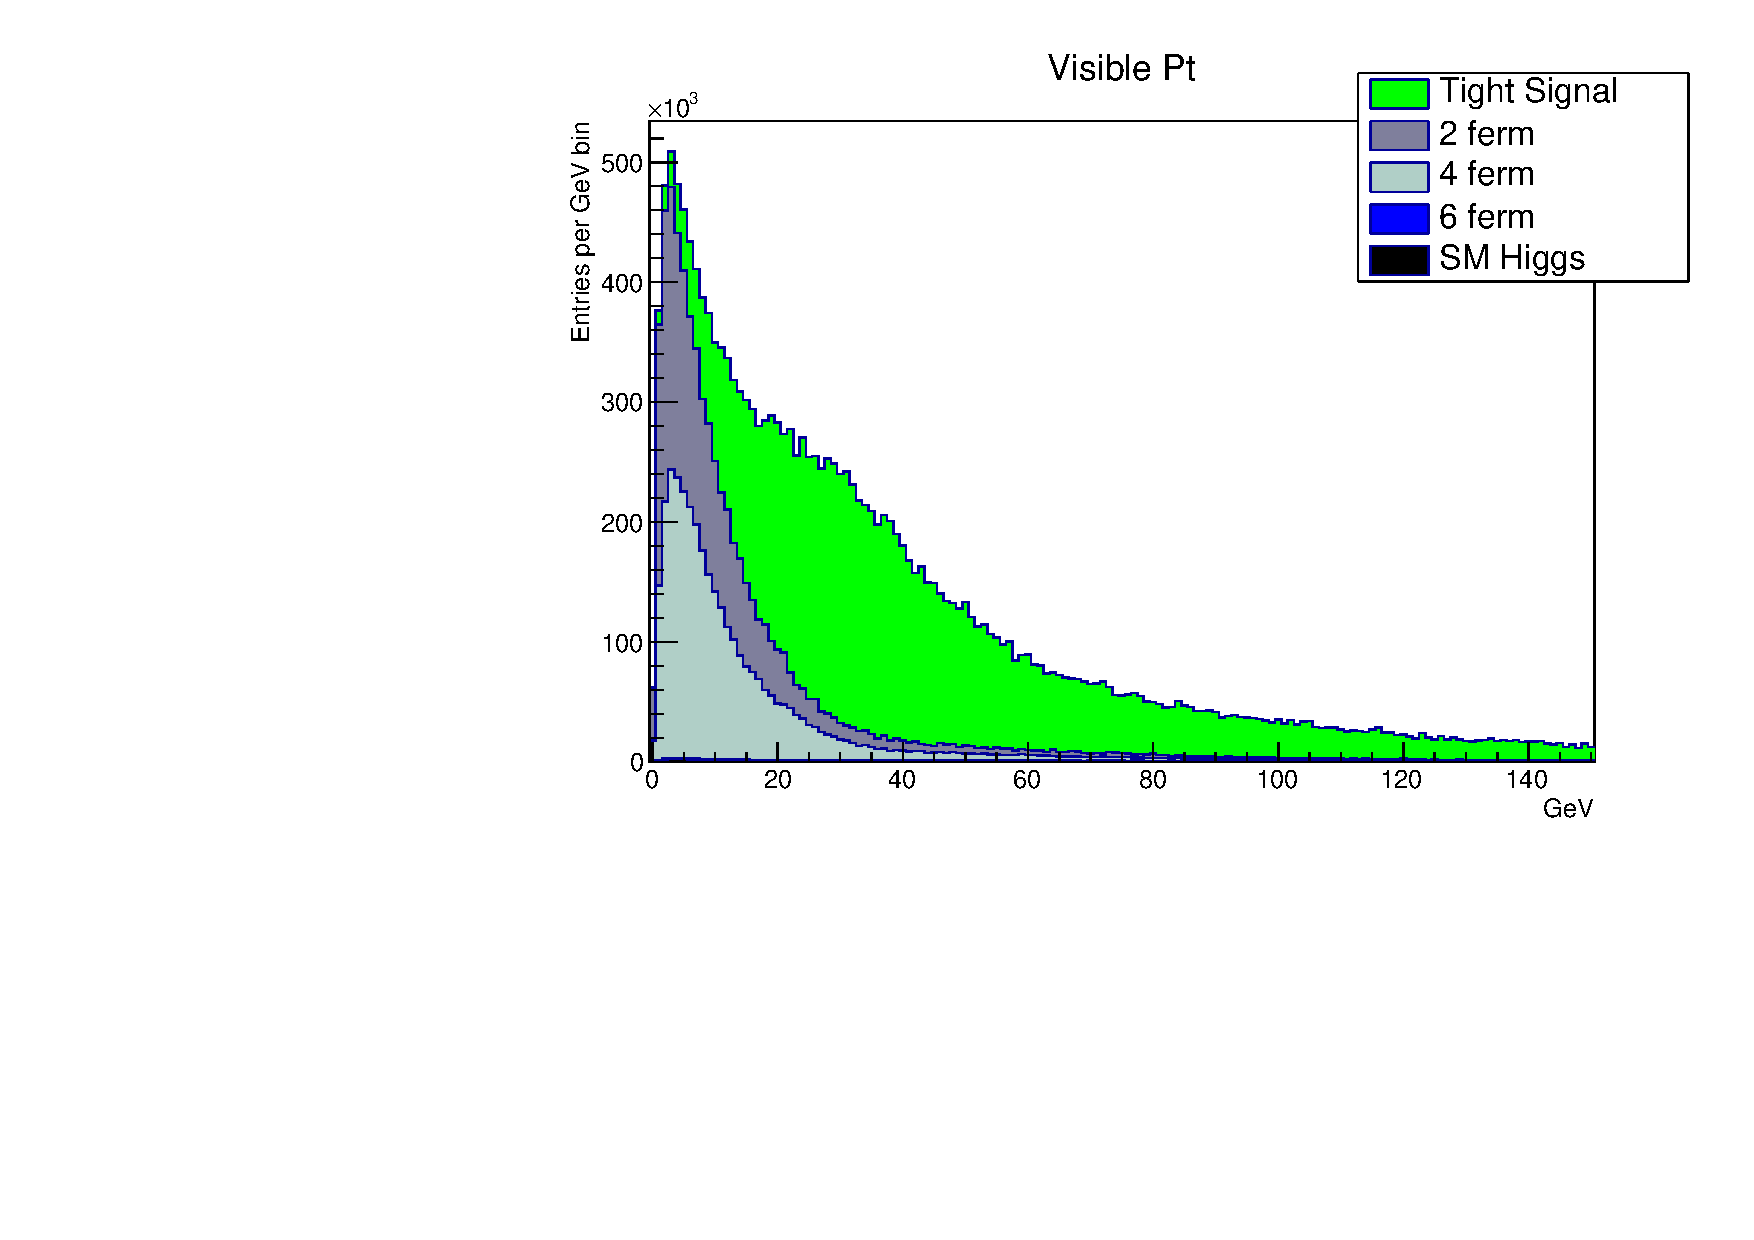
\includegraphics[scale=0.3, left]{PtvisHist.pdf} \\
N Leptons $> 0$
\end{column}
\begin{column}{0.5\textwidth}
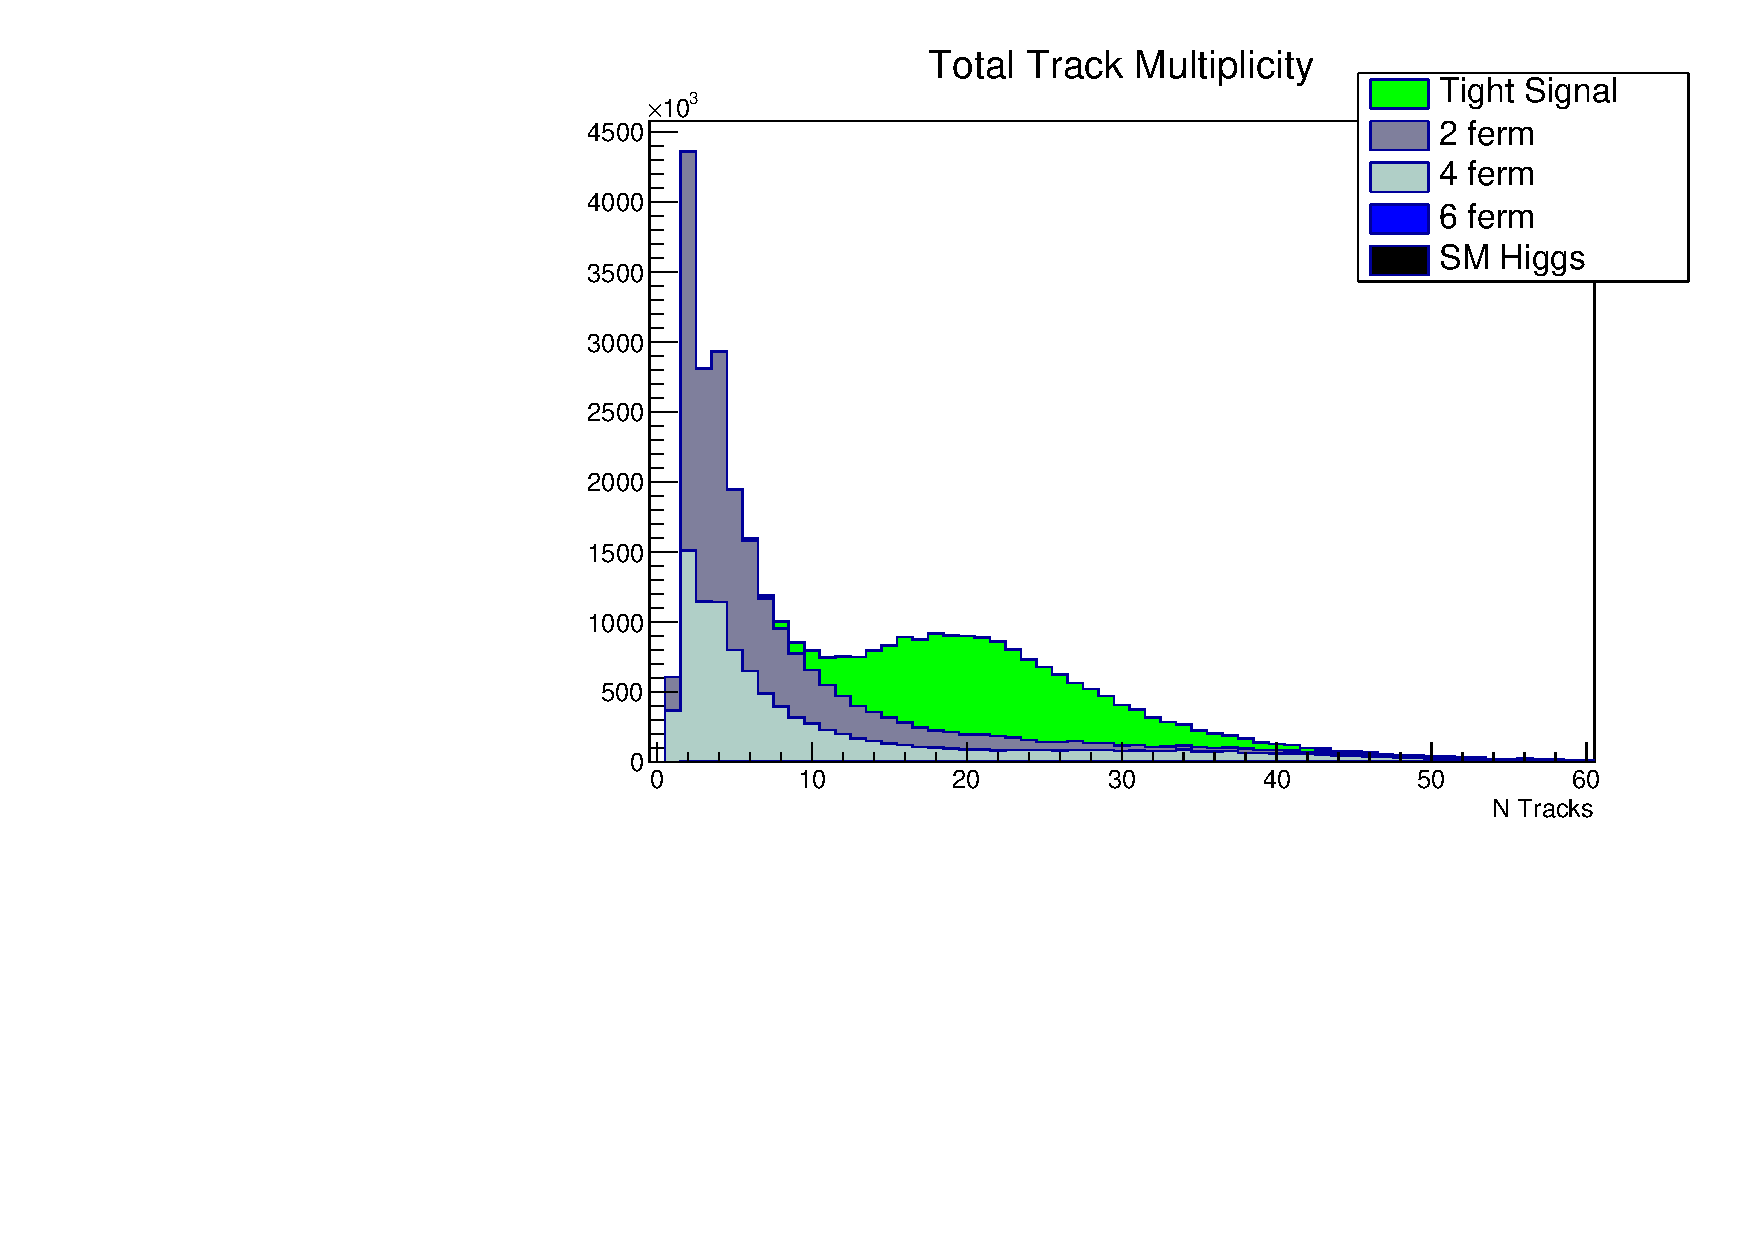
\includegraphics[scale=0.3, left]{ntracksHist.pdf} \\
N Tracks $> 10$
\end{column}
\end{columns}
\end{frame}



\begin{frame}{(3) Event Selection (Tight)}

Hadronic Mass Before and After all cuts\\
\scriptsize
Tight Signal $\Rightarrow$  muon cone for $\mu,e,\tau$ signal events\\
Left plot includes an N Lepton $> 0$ cut\\
Polarization: (-0.8,+0.3)\quad
Luminosity: 1600 fb$^{-1}$
(Includes off-shell types of events)
\begin{columns}
\begin{column}{0.5\textwidth}
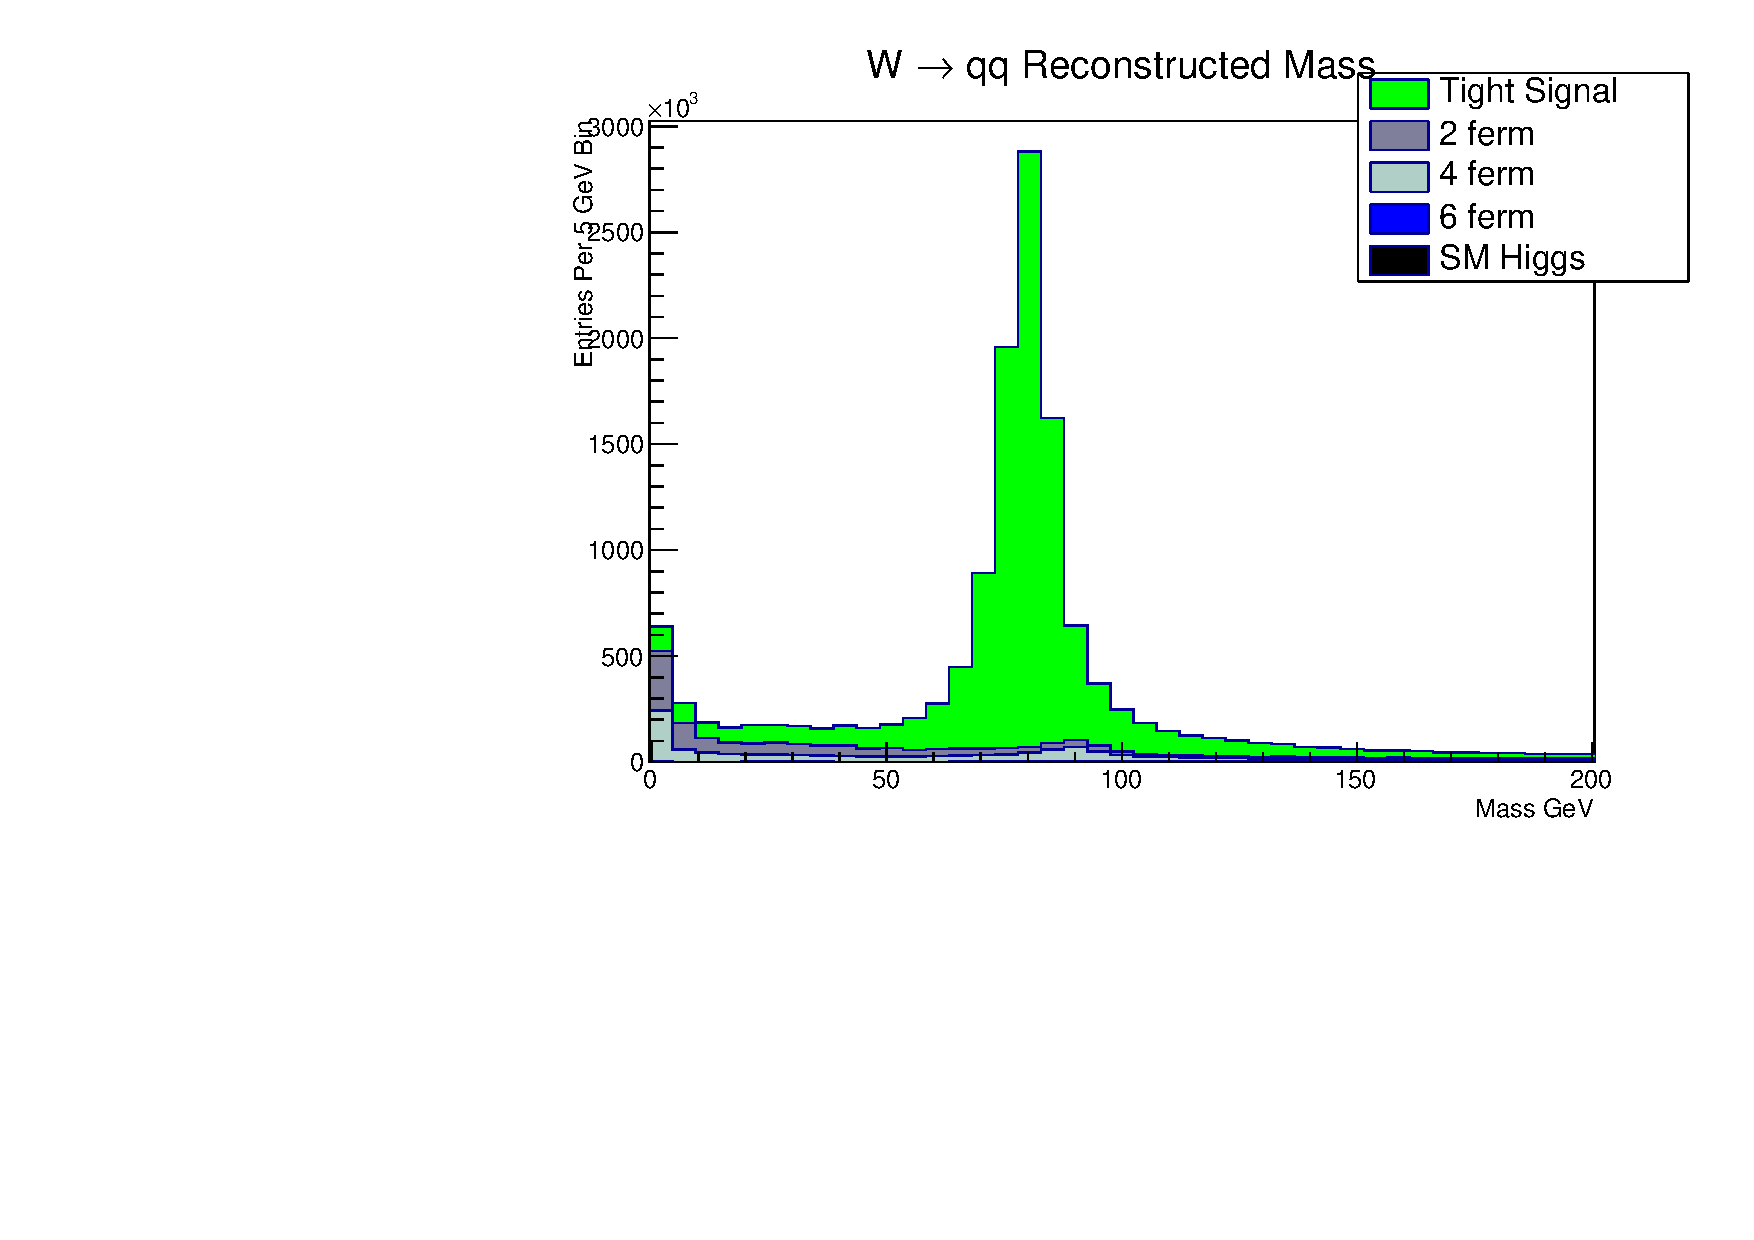
\includegraphics[scale=0.3, left]{mwhadHist.pdf} \\
$ 40 < M_{qq} < 120$
\end{column}
\begin{column}{0.5\textwidth}
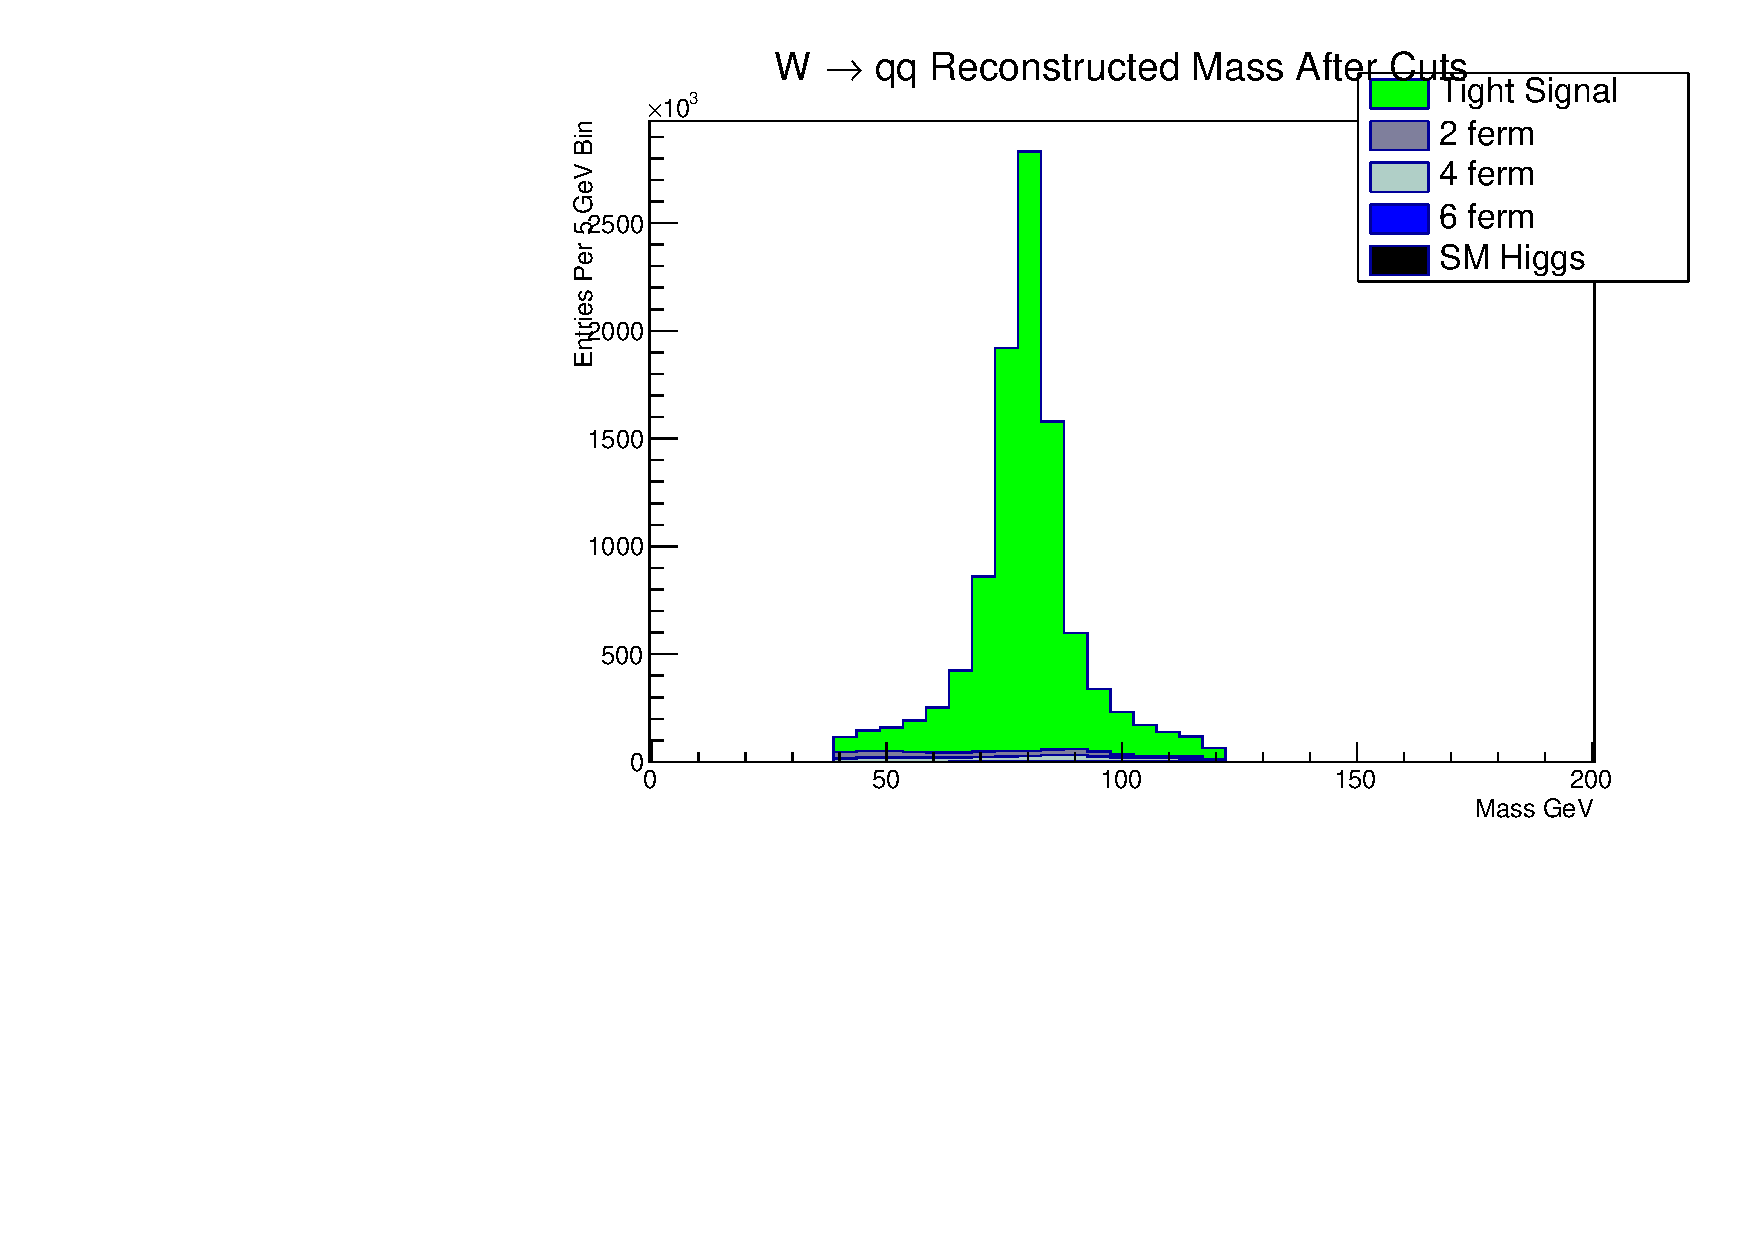
\includegraphics[scale=0.3, left]{mwhadCutsHist.pdf} \\

\end{column}
\end{columns}
\end{frame}



\begin{frame}{(3) Event Selection -- ``WW-like" Signal}
\scriptsize
Polarization: (-0.8,+0.3)\quad
Luminosity: 1600 fb$^{-1}$
\makebox[\linewidth]{\parbox{12.5cm}{  %}}
\tiny
Tight Selection with muon cone\\
   \begin{tabular}{|p{0.09\textwidth}p{0.08\textwidth}p{0.08\textwidth}p{0.08\textwidth}p{0.08\textwidth}p{0.08\textwidth}p{0.08\textwidth}p{0.08\textwidth}p{0.08\textwidth}|}
\hline 
   & Prompt $\mu$ & Prompt $e$ & $\tau$ & Tot. Sig. & 2f & 4f & 6f & Higgs \\ \hline 
Base Evts &\num{3.87e+06 } & \num{3.89e+06 } & \num{3.90e+06} &\num{1.17e+07} & \num{4.22e+07} & \num{3.22e+07} & \num{2.14e+05} & \num{4.12e+05} \\ 

Lepton &\num{3.31e+06 } & \num{3.20e+06 } & \num{2.28e+06} &\num{8.78e+06} & \num{1.15e+07} & \num{1.18e+07} & \num{1.63e+05} & \num{1.15e+05} \\ 
 
$E_{vis}$ &\num{3.28e+06 } & \num{3.11e+06 } & \num{2.27e+06} &\num{8.67e+06} & \num{1.06e+07} & \num{1.15e+07} & \num{1.62e+05} & \num{1.11e+05} \\ 
 
N Tracks &\num{3.19e+06 } & \num{3.03e+06 } & \num{2.21e+06} &\num{8.43e+06} & \num{2.54e+06} & \num{2.59e+06} & \num{1.49e+05} & \num{8.89e+04} \\ 
 
$-qcos\theta$ &\num{3.18e+06 } & \num{3.01e+06 } & \num{2.18e+06} &\num{8.37e+06} & \num{2.19e+06} & \num{2.26e+06} & \num{1.44e+05} & \num{8.52e+04} \\ 
 
$M_{qq}$ $>$40 &\num{2.94e+06 } & \num{2.80e+06 } & \num{2.03e+06} &\num{7.77e+06} & \num{1.13e+06} & \num{1.33e+06} & \num{1.42e+05} & \num{7.56e+04} \\ 
 
$M_{qq}$ $<$120 &\num{2.72e+06 } & \num{2.57e+06 } & \num{1.83e+06} &\num{7.13e+06} & \num{5.68e+05} & \num{2.68e+05} & \num{2.02e+04} & \num{2.97e+04} \\ 
 
$E_{com}$ &\num{2.72e+06 } & \num{2.57e+06 } & \num{1.83e+06} &\num{7.13e+06} & \num{5.58e+05} & \num{2.65e+05} & \num{2.02e+04} & \num{2.96e+04} \\ 

Pt vis. &\num{2.69e+06 } & \num{2.55e+06 } & \num{1.81e+06} &\num{7.05e+06} & \num{3.21e+05} & \num{2.37e+05} & \num{2.01e+04} & \num{2.94e+04} \\ 

$m^2_{\nu recoil}$ &\num{2.69e+06 } & \num{2.54e+06 } & \num{1.80e+06} &\num{7.03e+06} & \num{2.93e+05} & \num{2.02e+05} & \num{1.94e+04} & \num{2.23e+04} \\ 
\hline 
\rowcolor{green}
 $\epsilon$ & $0.6944 \pm 0.0024$ & $0.6542 \pm 0.0023$ & $0.4616 \pm 0.0027$ &  $0.6032 \pm 0.0015$ & $0.006941 \pm 0.00012$ & $0.006255 \pm 7.6e-05$ & $0.09051 \pm 0.00023$ & $0.05407 \pm 0.00045$ \\ 
\hline
\end{tabular}
\quad \quad \\
Loose selection with tau cone\\
\begin{tabular}{|p{0.09\textwidth}p{0.08\textwidth}p{0.08\textwidth}p{0.08\textwidth}p{0.08\textwidth}p{0.08\textwidth}p{0.08\textwidth}p{0.08\textwidth}p{0.08\textwidth}|}
\hline 
   & Prompt $\mu$ & Prompt $e$ & $\tau$ & Tot. Sig. & 2f & 4f & 6f & Higgs \\ \hline 
Base Evts &\num{3.87e+06 } & \num{3.89e+06 } & \num{3.90e+06} &\num{1.17e+07} & \num{4.22e+07} & \num{3.22e+07} & \num{2.14e+05} & \num{4.12e+05} \\ 
 
Lepton &\num{3.36e+06 } & \num{3.30e+06 } & \num{2.82e+06} &\num{9.48e+06} & \num{1.30e+07} & \num{1.36e+07} & \num{1.77e+05} & \num{1.38e+05} \\ 

Tight Lep. Veto &\num{7.72e+04 } & \num{1.28e+05 } & \num{5.70e+05} &\num{7.76e+05} & \num{1.93e+06} & \num{2.15e+06} & \num{1.61e+04} & \num{3.12e+04} \\ 
 
$E_{vis}$ &\num{7.64e+04 } & \num{1.26e+05 } & \num{5.70e+05} &\num{7.72e+05} & \num{1.82e+06} & \num{1.94e+06} & \num{1.54e+04} & \num{3.02e+04} \\ 

N Tracks &\num{7.37e+04 } & \num{1.21e+05 } & \num{5.54e+05} &\num{7.49e+05} & \num{1.50e+06} & \num{1.64e+06} & \num{1.51e+04} & \num{2.71e+04} \\ 
 
$-qcos\theta$ &\num{6.30e+04 } & \num{1.12e+05 } & \num{5.32e+05} &\num{7.07e+05} & \num{1.11e+06} & \num{1.41e+06} & \num{1.45e+04} & \num{2.56e+04} \\ 
 
$M_{qq}$ $>$ 40 &\num{4.92e+04 } & \num{9.72e+04 } & \num{4.86e+05} &\num{6.33e+05} & \num{5.98e+05} & \num{1.30e+06} & \num{1.44e+04} & \num{2.33e+04} \\ 

$M_{qq}$ $<$ 120 &\num{4.04e+04 } & \num{7.81e+04 } & \num{4.16e+05} &\num{5.35e+05} & \num{2.58e+05} & \num{1.11e+05} & \num{1.11e+03} & \num{1.24e+04} \\ 
 
$E_{com}$ &\num{4.04e+04 } & \num{7.81e+04 } & \num{4.16e+05} &\num{5.34e+05} & \num{2.50e+05} & \num{1.10e+05} & \num{1.11e+03} & \num{1.24e+04} \\ 

Pt vis. &\num{4.00e+04 } & \num{7.74e+04 } & \num{4.12e+05} &\num{5.29e+05} & \num{1.17e+05} & \num{1.01e+05} & \num{1.11e+03} & \num{1.23e+04} \\ 
 
$m^2_{\nu recoil}$ &\num{3.94e+04 } & \num{7.70e+04 } & \num{4.07e+05} &\num{5.24e+05} & \num{1.02e+05} & \num{7.59e+04} & \num{1.02e+03} & \num{9.73e+03} \\ 
\hline 
\rowcolor{emerald}
 $\epsilon$ & $0.01017 \pm 0.00053$ & $0.01982 \pm 0.00071$ & $0.1046 \pm 0.0018$ &  $0.04495 \pm 0.00065$ & $0.002411 \pm 3.2e-05$ & $0.002356 \pm 3.7e-05$ & $0.004742 \pm 6.7e-05$ & $0.0236 \pm 0.00024$ \\ 


 \hline
 \end{tabular}

%end box
}}
\end{frame}


\begin{frame}{Event Selection Summary (LR)}
 \tiny
 (-0.8, +0.3) 1600 fb${^-1}$\\
  \begin{tabular}{ |p{0.08\textwidth}|p{0.08\textwidth}p{0.08\textwidth}|p{0.08\textwidth}|p{0.08\textwidth}p{0.08\textwidth}p{0.08\textwidth}|} 
 \hline 
   &  \multicolumn{3}{|l|}{Tight Selection} &  \multicolumn{3}{|l|}{ Tight + Loose Sel.}  \\  \hline  
 & Sel. Total & Efficiency & Purity & Sel. Total & Efficiency & Purity \\ 
 \hline  
 Bkg. & 5.36e+05 & & & 7.25e+05 & &  \\ 
 Signal & 4.49e+06 & 0.578 $\pm$ 0.002 & 0.893  & 4.93e+06 & 0.635 $\pm$ 0.002 & 0.872 \\ 
 \rowcolor{orange}
 Sig.+O.S. & 6.93e+06 & 0.541 $\pm$ 0.001 & 0.928 & 7.47e+06 & 0.584 $\pm$ 0.001 & 0.912 \\ 
\hline 
\end{tabular} 
 \\
\normalsize
\quad \quad \\
\scriptsize
\begin{itemize}
\item[-] Signal is only on-shell WW-like events
\item[-] Signal + O.S.(Off-Shell) includes both selections including the not WW-like signal events
\item[-] in LR we find ratio of S/B to be 1 order of magnitude
\item[-] Good efficiency and high purity for the signal case
\item[-] When adding O.S. events we only strengthen the purity, but efficiency drops because the events are not ideal for selection
\end{itemize}
With Sig.+O.S. and Tight + Loose Sel.\\
\colorbox{yellow}{ $ \frac{\Delta\sigma}{\sigma} (stat.) = 0.04 \%$}
\end{frame}

\begin{frame}{(4) W-Mass Measurement }
Comparison of Generator mass differences\\
Before $\&$ After  pileup removal and selection cuts \\
Polarization: (-0.8,+0.3)\quad
Luminosity: 1600 fb$^{-1}$\\

\begin{center}
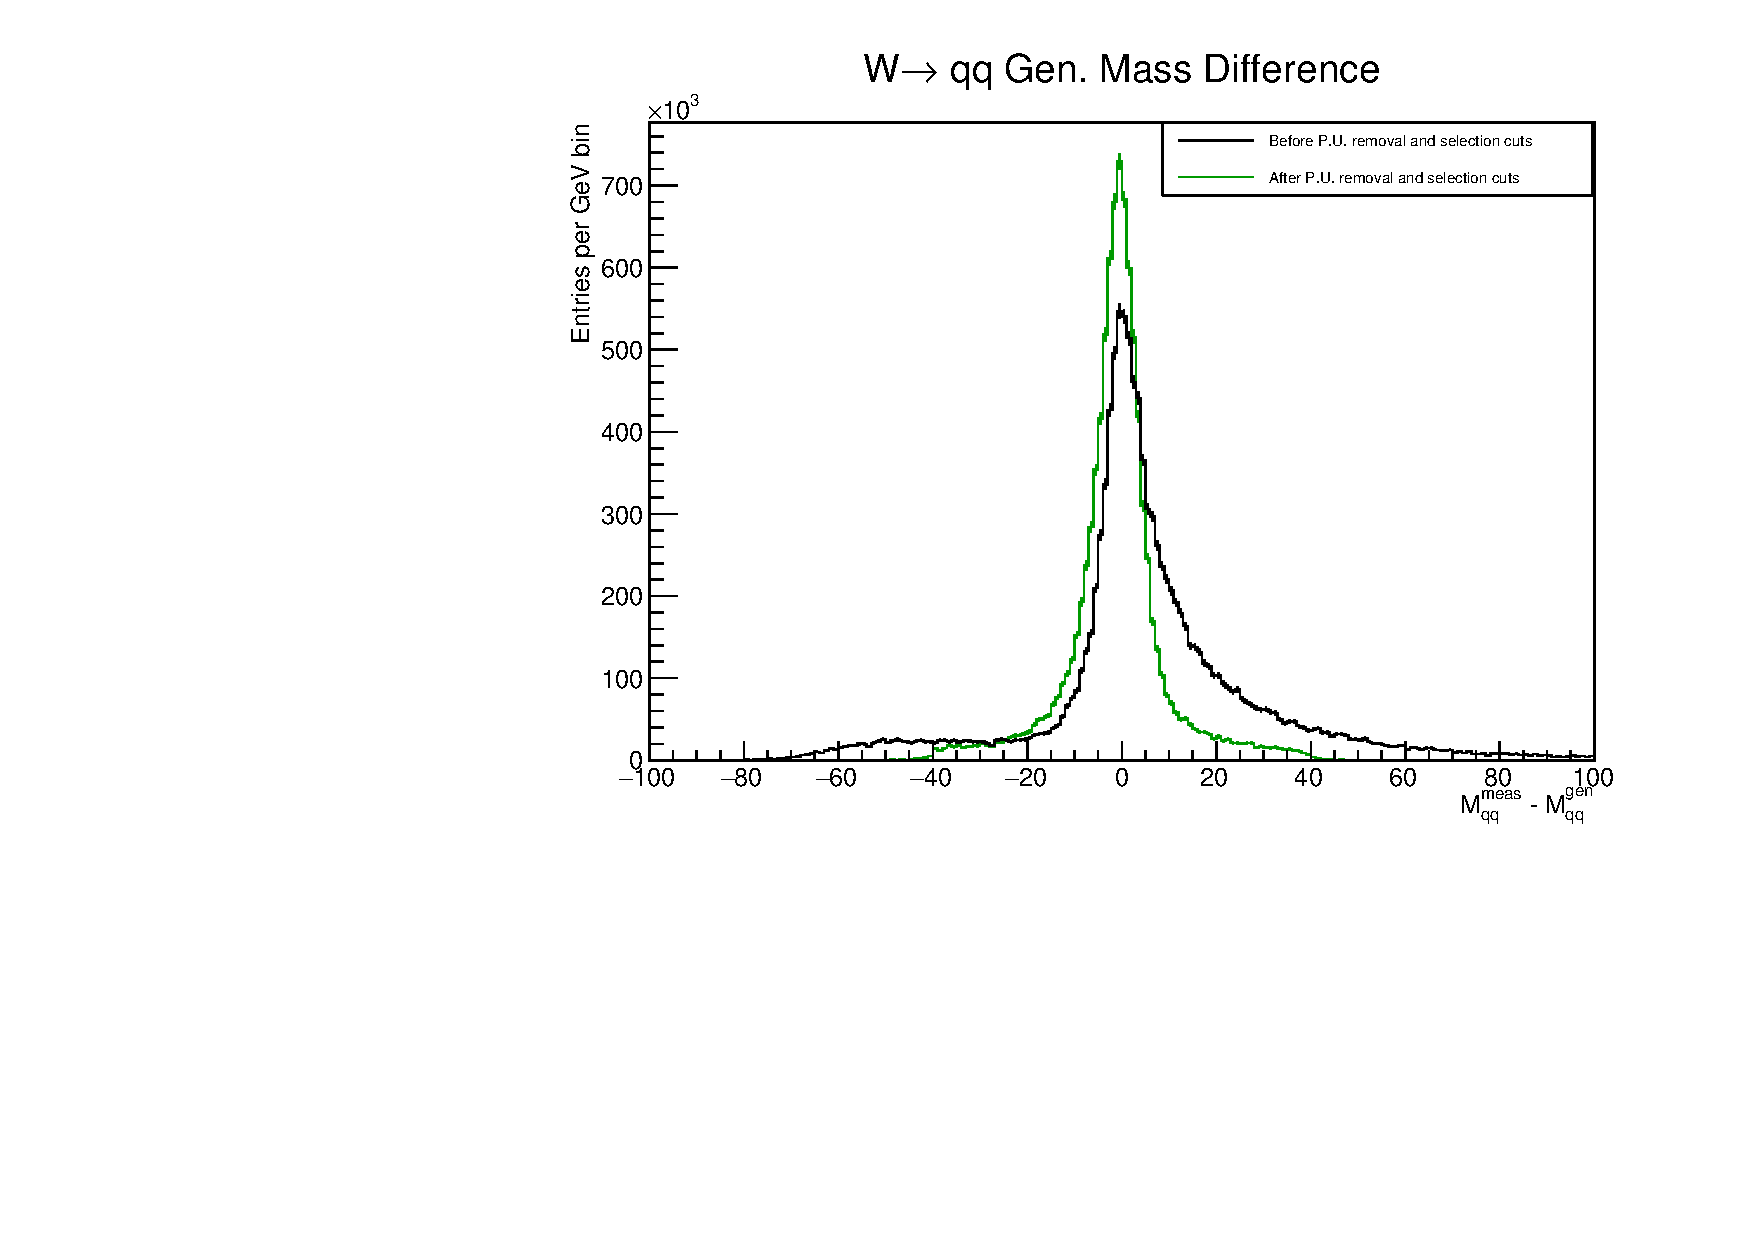
\includegraphics[scale=0.4]{moneymassdiff.pdf} \\
\end{center}


\end{frame}
\begin{frame}{(4) W-Mass Measurement }
\scriptsize
Polarization: (-0.8,+0.3)\quad
Luminosity: 1600 fb$^{-1}$\\
Tight Signal+O.S. $\mu ,\tau , e$\\
\scriptsize
\begin{columns}
\begin{column}{0.5\textwidth}

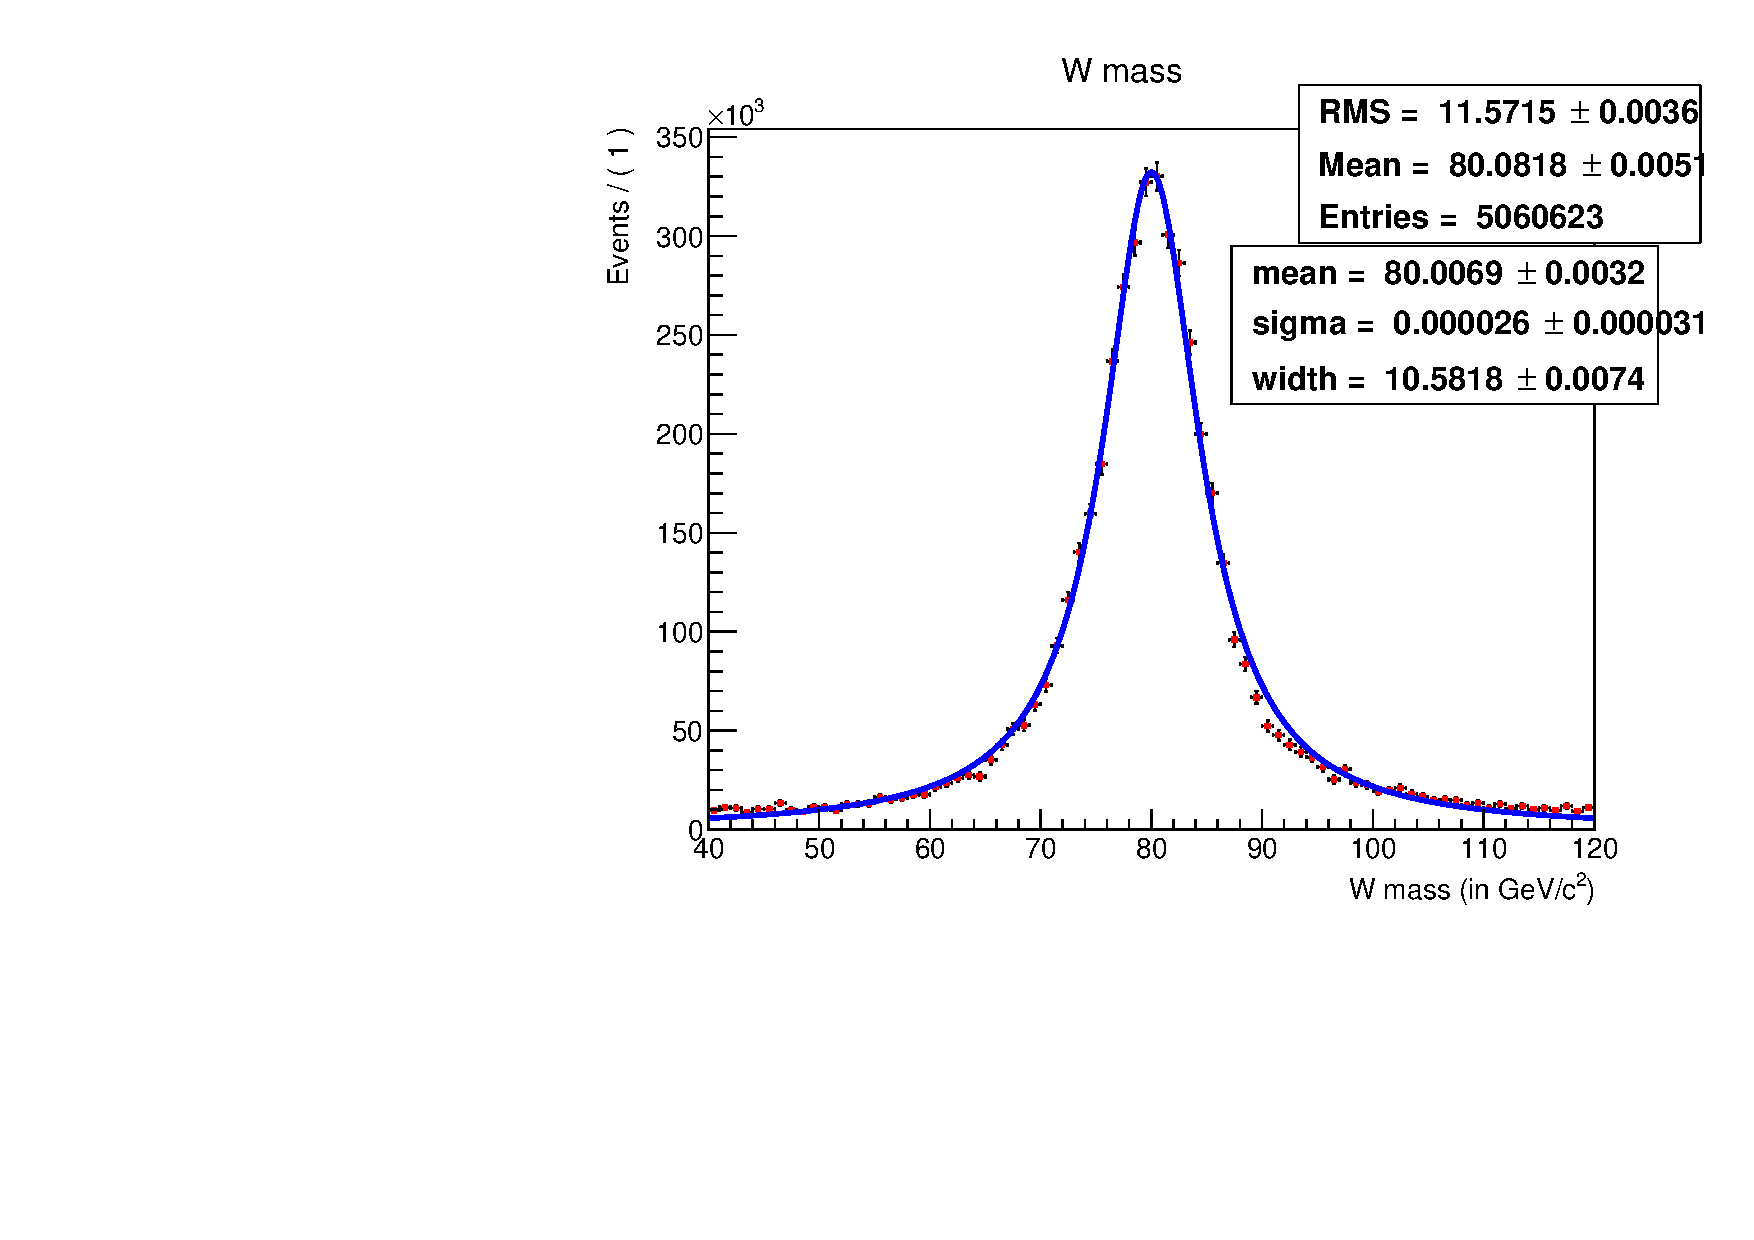
\includegraphics[scale=0.3, left]{WWSfit.pdf} \\
\begin{itemize}
\scriptsize
\item Applied Voigtian fit to get a model for W-mass shape
\item Poor fit, and statistical errors correspond to unweighted number of events
\item Fit params. $M_W = 79.7074$ GeV, width $\Gamma_W = 10.6972$ GeV and $\sigma_W = 4.847e-7$ GeV
\end{itemize}
\end{column}
\begin{column}{0.5\textwidth}

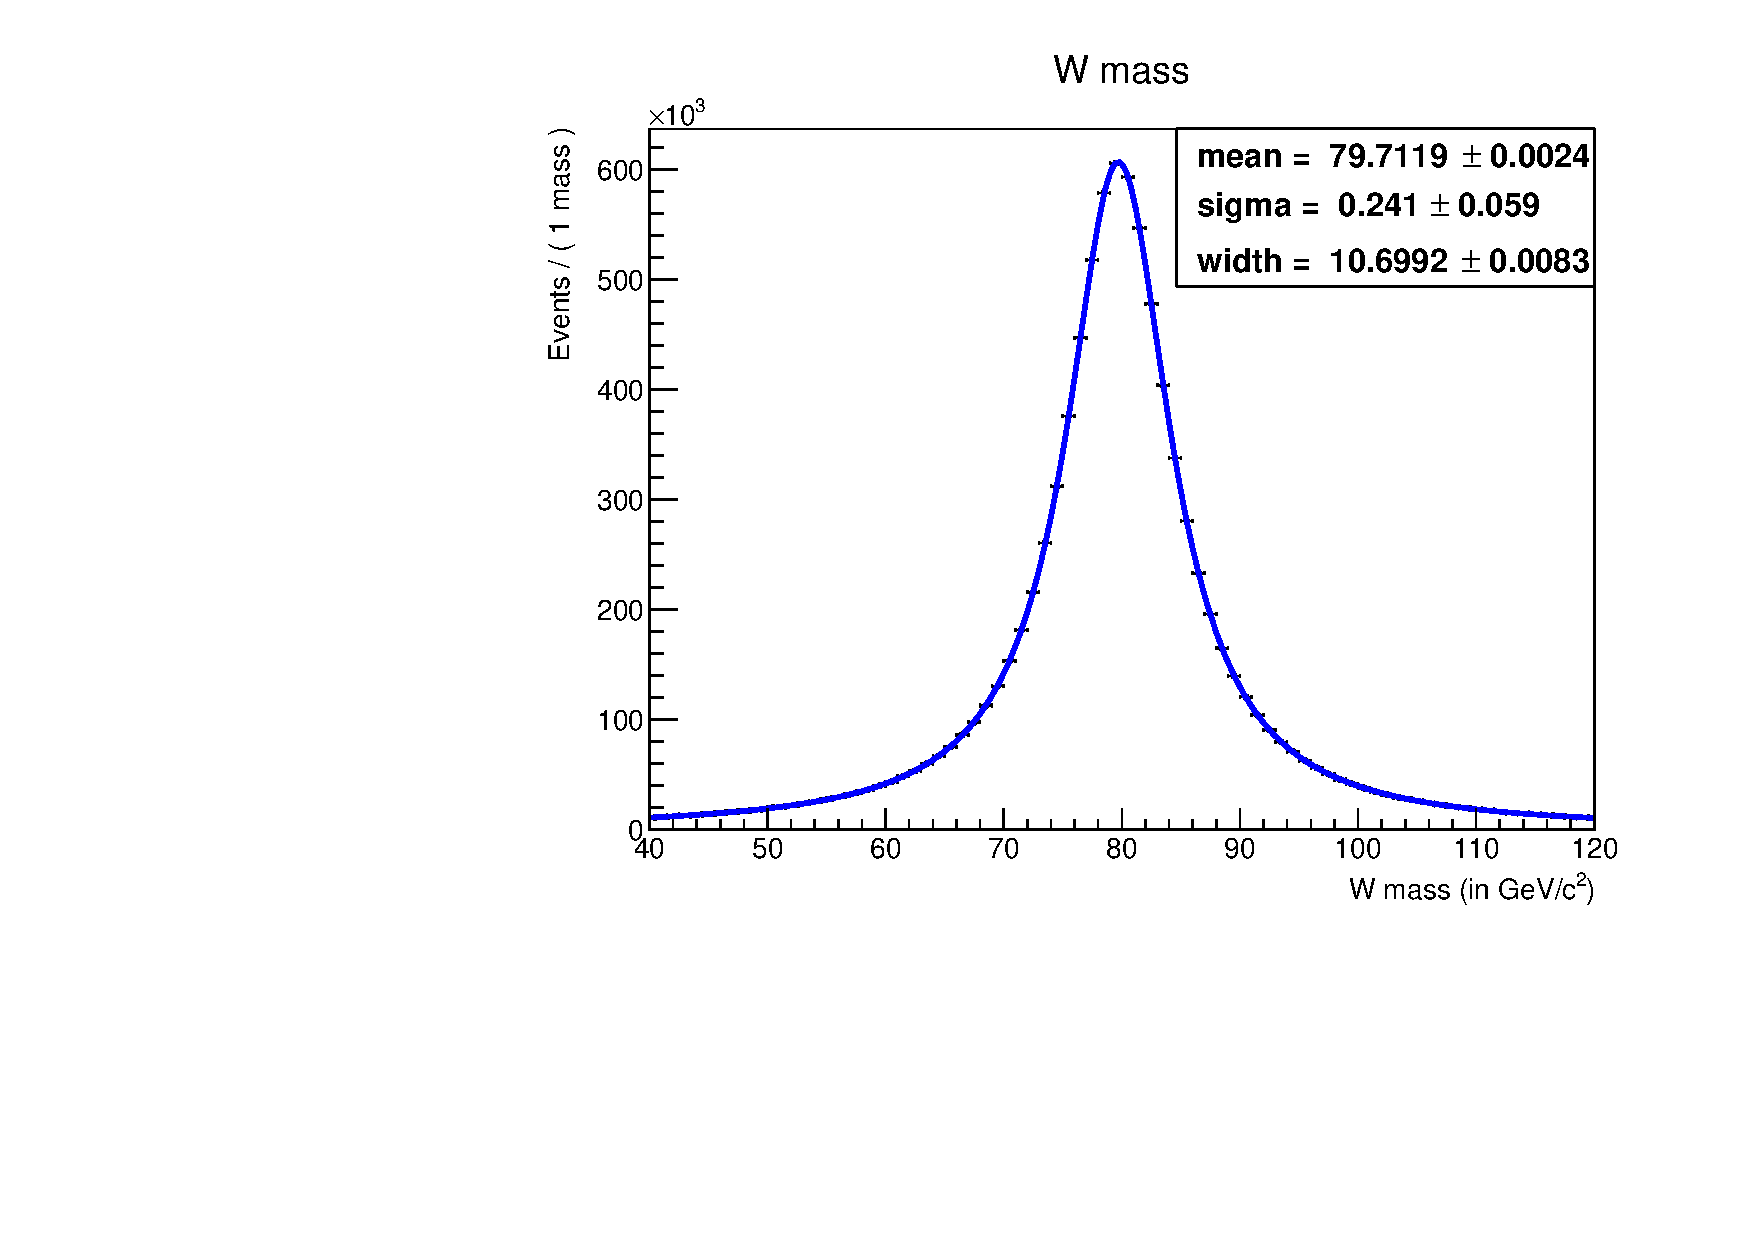
\includegraphics[scale=0.3, left]{Wtoyfit.pdf} \\
\begin{itemize}
\item Fit a toy model based on previous shape fit
\item Uses statistics of 1600 fb$^{-1}$ (9M Events)
\item \colorbox{green}{$\Delta M_W (\text{stat.}) = 2.4 \, \text{MeV} \, \, \chi^2/ndof = 67.8/77$ }
\item Estimate with good systematics $\rightarrow$ $\Delta M_W = 4.6$ MeV
\item Current PDG value: $\Delta M_W = 12$ MeV
\end{itemize}
\end{column}
\end{columns}
\quad \quad \\
\quad \quad \\

\end{frame}


\begin{frame}{Summary}
\scriptsize
Completed Work:
\begin{itemize}
	\item[-] Performed a benchmarking analysis with $WW\rightarrow qq\ell\nu$
	\item[-] Treated the leptons universally with TauFinder
	\item[-] Rejected $\gamma \gamma$ pileup by fragmenting jets and making a Pt cut on the resulting mini-jets
	\item[-] Performed a basic event selection for main polarization with 1600 fb$^{-1}$ of data
	\item[-] Reported statistical errors $\Delta M_W$ and $\Delta\sigma$
	
\end{itemize}
TODO:
\begin{itemize}
	\item[-] Constrained fitting for W-mass and event selection improvements
	\item[-] Study efficiency as a function of $cos\theta$ of the lepton 
	\item[-] Separate muonic taus and prompt muons using IP significance or constrained fits
	\item[-] Do analysis at $\sqrt{s} = 250$ GeV

\end{itemize}
Future Plans:
\begin{itemize}
	\item[-] ILC progress doesn't grant much incentive to continue work
	\item[-] Future focus: CMS exclusive
	\item[-] compressed SUSY search w/ leptons, hopefully with new ML type approaches to analysis

\end{itemize}

\end{frame}







\end{document}